\documentclass{jsarticle}
\usepackage[dvipdfmx]{graphicx}
\usepackage{ascmac}
\begin{document}
%%title
%\title{SHIMADA LAB. CODE\\MANUAL}
%\author{山中翔太}%{{{
%\maketitle
%\newpage
%\tableofcontents
%%}}}
%\newpage
%
%%tutorial
%\part{基本事項}
%\newpage
%\section{はじめに}%{{{
%本プログラムは「流体コード」「化学モデル」「0次元化学コード」の生成プログラムである。
%
%本章ではまずはじめに、「化学コードを用いたメタン/空気完全平衡モデル簡略化モデル作成」と「簡略モデルを用いた作動流体にメタンと空気を用いた衝撃波管問題」という二つの例題を解きながら、全てのコードに関わる重要事項について
%\begin{itembox}[l]{重要}
%このボックスを用いながら
%\end{itembox}
%説明する。
%
%そのあと、condition.f90で用いられる代表的な境界条件について説明する。
%
%最後に、デバッグに使える多少のコマンドについて説明する。
%
%\begin{itembox}[l]{環境条件}
%本プログラムはUbuntu 12.04 LTS上で正常な実行を確認している。
%
%また、以下のプログラムを用いている。
%\begin{itemize}
%\item intel fortran (non-commercial)
%\item python
%\item wx-python
%\end{itemize}
%使用する際には以上のプログラムをまずインストールすること。
%
%また、外部ライブラリとして
%\begin{itemize}
%\item dvode.f from ODEPACK
%\item thermo.inp from NASA-CEA
%\item trans.inp from NASA-CEA
%\end{itemize}
%を用いており、これらのファイルを再頒布している。
%\end{itembox}
%
%%}}}
%\newpage
%\section{チュートリアル}%{{{
%\subsection{化学コードを用いたメタン/空気完全平衡モデル簡略化モデル作成}%{{{
%この例題は"元モデルの作成"と"その簡略化"にわけられる。それぞれを説明する。
%\subsubsection{元モデルの作成}
%コードの生成はcheckout.pyでできるが、
%\begin{itembox}[l]{重要}
%checkout.pyでできる動作は全てGUI.pyを通して行うことができる。
%\end{itembox}
%よって、コード生成はGUI.pyを通して行うことをお勧めする。
%
%GUI.pyは以下のコマンドで起動される。
%\begin{itembox}[l]{重要}
%\begin{verbatim}
%./GUI.py
%\end{verbatim}
%\end{itembox}
%起動されると以下の画面が立ち上がる。
%\begin{center}
%\includegraphics[width=.7\textwidth,bb=0 0 895 649]{tutorial_img/010.png}
%\end{center}
%今回はまず元モデルの生成を行う。まずは上のタブで"chemical model"を選択する。
%\begin{center}
%\includegraphics[width=.7\textwidth,bb=0 0 895 649]{tutorial_img/020.png}
%\end{center}
%起動されたら、まずthermal modelで完全平衡モデル"NASA CEA"を選び、"Not Selected"の中から生成物として使いたい化学種をダブルクリックすることで選択する。今回はメタン空気の燃焼なので、CH4,N2,O2の三つを選べばよい。なお、この際"Not Selected"内でCtrl+Fをうつと検索モードとなり、所望の化学種を素早くみつけることができる。
%\begin{center}
%\includegraphics[width=.7\textwidth,bb=0 0 895 649]{tutorial_img/030.png}
%\includegraphics[width=.7\textwidth,bb=0 0 895 649]{tutorial_img/035.png}
%\end{center}
%選び終えたら"Generate CODE!"を押下すると、コードが生成される。
%\begin{center}
%\includegraphics[width=.3\textwidth,bb=0 0 268 174]{tutorial_img/040.png}
%\end{center}
%\begin{itembox}[l]{重要}
%流体コード生成、化学コード生成の場合でも、"exit value:0"が正常終了である。
%"***********"の行から"***********"の行までがコード生成の際に生成されたメッセージとなるので、正常終了しなかった場合にはこのメッセージを読んで対策を講じること。
%\end{itembox}
%上の例の場合はコード生成の際にメッセージは生成していない。
%
%以上の動作を終えるとディレクトリに"chem.inp"と"control\_chem.raw.inp"が生成される。
%\begin{itembox}[l]{重要}
%熱力学モデルが理想気体でない場合、化学コードでも流体コードでも、コード生成の際にはcheckout.pyと同じ階層に使用されるchem.inpを配置する必要があり、また生成したコードを走らせる際には"control\_chem.raw.inp"を編集し"control\_chem.inp"として実行ファイルと同じ階層に配置する必要がある。
%
%NASAデータベースを用いる際には"control\_chem.inp"の雛形はこの操作でしか生成しないので取扱いに気をつけること。
%\end{itembox}
%
%\subsubsection{モデルの簡略化}
%続けて化学コードの生成を行う。このためにはGUI.pyの上のタブで"chemical calculation"を選ぶ。
%\begin{center}
%\includegraphics[width=.7\textwidth,bb=0 0 895 649]{tutorial_img/050.png}
%\end{center}
%図のように
%\begin{itemize}
%\item thermal model : NASA CEA
%\item calc model : reduction
%\item constants : constant pressure and enthalpy
%\end{itemize}
%を選んだら"Generate CODE!"を押下する。
%\begin{itembox}[l]{重要}
%この際、"chem.inp"が"checkout.py"と同じ階層にいなければ異常終了するので注意すること。
%\end{itembox}
%\begin{center}
%\includegraphics[width=.4\textwidth,bb=0 0 380 327]{tutorial_img/060.png}
%\end{center}
%コード生成時の"checkout.py"からのメッセージから適切な設定が生成されたこと、また"exit value:0"からコード生成に成功したことがわかる。ここでOKを押すと、自動的にGUI.pyが閉じられる。
%
%以上の動作を行うと、ディレクトリは以下のようになる。
%\begin{center}
%\includegraphics[width=.8\textwidth,bb=0 0 962 577]{tutorial_img/070.png}
%\end{center}
%checkout\_chemが新たに生成されていることが分かる。
%
%ここで、control\_chem.raw.inpを以下のように設定する。
%\begin{center}
%\includegraphics[width=.8\textwidth,bb=0 0 962 577]{tutorial_img/080.png}
%\end{center}
%control\_chem.inpは燃料と酸化剤それぞれの組成、圧力、初期温度、必要な場合は生成物の組成と時間積分ライブラリに使うパラメータを設定する。今回は完全平衡モデルであるので本来ならばProductsの欄はいらないが、流体に用いるために定義しておく。詳しい書式は\ref{store/therm_lib/NASA}に記載している。
%以上のように設定できたらcontrol\_chem.raw.inpをcontrol\_chem.inpに名前変更し、checkout\_chemにコピーする。するとcheckout\_chemの中身は以下のようになる。
%\begin{center}
%\includegraphics[width=.8\textwidth,bb=0 0 962 577]{tutorial_img/090.png}
%\end{center}
%ここにもcontrol.raw.inpという"raw"がつくファイルがあるので、適切に編集したあとcontrol.inpに変更しなければならない。
%\begin{itembox}[l]{重要}
%このように、"raw"がつくファイルが生成した場合には、適切に編集の上"raw"をとったファイル名に名前変更しなければならない。
%\end{itembox}
%このようなファイルには他にcondition.raw.f90がある。
%
%control.inpは以下のように変更する。
%\begin{center}
%\includegraphics[width=.8\textwidth,bb=0 0 962 577]{tutorial_img/095.png}
%\end{center}
%詳細な書式は\ref{NASA/reduction}参照のこと。
%以上の編集がおわったら、control.raw.inpをcontrol.inpに変更する。
%\begin{center}
%\includegraphics[width=.8\textwidth,bb=0 0 962 577]{tutorial_img/100.png}
%\end{center}
%ここまで終了したらmakeコマンド
%\begin{verbatim}
%make
%\end{verbatim}
%をうつ。するとコードがコンパイルされるので
%\begin{verbatim}
%./driver
%\end{verbatim}
%を実行すると、以下のように出力される。
%\begin{center}
%\includegraphics[width=.8\textwidth,bb=0 0 962 577]{tutorial_img/110.png}
%\end{center}
%ここから、元々のモデルでは158あった化学種が7まで削減され、また最大温度誤差が1.7\%であることがわかる。
%
%\begin{itembox}[l]{重要}
%なお、実行ファイルは流体コードでは"main"、化学コードでは"driver"である。
%\end{itembox}
%
%ここで生成されたファイルはchem.inp.newというファイルで保存される。chem.inp.newのファイルの中は以下のようになっている。
%\begin{center}
%\includegraphics[width=.8\textwidth,bb=0 0 962 577]{tutorial_img/120.png}
%\end{center}
%ここから、僅か7つの化学種のみが用いられていることがわかる。これをchem.inpと名前変更して使用すると、元モデルの代わりに簡略モデルを用いることができる。
%%}}}
%\subsection{簡略モデルを用いた作動流体にメタンと空気を用いた衝撃波管問題}%{{{
%前節が終わった時点でcheckout.pyと同じ階層にあるchem.inpには158化学種存在する。これを簡略化モデルに置き換えるにはcheckout.pyと同じ階層で
%\begin{verbatim}
%cp checkout_chem/chem.inp.new chem.inp
%\end{verbatim}
%などのコマンドをうつなどして、checkout\_chemで生成したchem.inp.newでcheckout.pyと同じ階層にあるchem.inpを置き換えればよい。
%
%流体コードを生成するには、また\verb|./GUI.py|でGUIを起動すればよい。
%\begin{center}
%\includegraphics[width=.8\textwidth,bb=0 0 895 649]{tutorial_img/130.png}
%\end{center}
%まずはGrid File Nameでグリッドを選ぶ。"Choose File"を押下すれば、ファイル選択画面が現れる。
%本チュートリアルではsample/no00.shock\_tube/debug0.xを選択する。
%\begin{center}
%\includegraphics[width=.8\textwidth,bb=0 0 842 659]{tutorial_img/140.png}
%\end{center}
%グリッドファイル選択後は
%\begin{itemize}
%\item Maximum Number of Processors : 0
%\item dimension : two dimension
%\item time scale : global
%\item time scheme : Euler
%\item high order scheme : MUSCL
%\item viscosity : viscous flow
%\item thermal model : Perfect Equilibrium Model
%\end{itemize}
%を選ぶ。それぞれの詳しい意味はsection \ref{流体コード}参照のこと。
%\begin{center}
%\includegraphics[width=.8\textwidth,bb=0 0 895 649]{tutorial_img/150.png}
%\end{center}
%この状態で"Generate CODE!"を押下すると以下のようなメッセージがでてくる。このメッセージから、正常終了していること(Exit Value: 0)、所望の機能が生成されていることがわかる。
%\begin{center}
%\includegraphics[width=.5\textwidth,bb=0 0 364 446]{tutorial_img/160.png}
%\end{center}
%\begin{itembox}[l]{重要}
%この際に、checkoutディレクトリ生成以前に元々checkoutディレクトリが存在する場合、その中に存在するcontrol.inpとcondition.f90、gridディレクトリについてはそれぞれcontrol.bak.inp、condition.bak.f90、grid\_bakディレクトリとしてバックアップがcheckout.pyと同じ階層にとられる。
%\end{itembox}
%
%以上の操作を行うと、checkoutディレクトリが生成し、中身が以下のようになる。
%\begin{center}
%\includegraphics[width=.8\textwidth,bb=0 0 962 577]{tutorial_img/170.png}
%\end{center}
%まず、NASAライブラリを使っているので、前述のとおりcontrol\_chem.inpをコピーしてくる必要がある。
%よって、簡略化の際用いたファイルをコピーしてくる。
%\begin{center}
%\includegraphics[width=.8\textwidth,bb=0 0 962 577]{tutorial_img/180.png}
%\end{center}
%また、前述のとおり"raw"がついているものを編集しなければならない。今回はcontrol.inpとcondition.f90である。
%control.inpは以下のように編集する。
%\begin{center}
%\includegraphics[width=.8\textwidth,bb=0 0 962 577]{tutorial_img/190.png}
%\end{center}
%これも詳しい書式はsection \ref{流体コード}参照のこと。
%
%\begin{itembox}[l]{重要}
%condition.f90については、一般的に
%\begin{itemize}
%\item 初期条件(set\_IC)
%\begin{itemize}
%\item q全て...保存量全て
%\item $w_4$...圧力
%\item $w_{indxg}$...比熱比
%\item $w_{indxR}$...気体定数
%\end{itemize}
%\item 境界条件(set\_BC)
%\begin{itemize}
%\item w全て...基本量及び、比熱比、気体定数、質量あたり全エンタルピー、粘性係数
%\item vhi全て...それぞれの気体グループの質量あたり内部エンタルピー
%\item Yv全て(NASAデータベース使用の場合)...それぞれの気体グループの質量分率
%\end{itemize}
%\end{itemize}
%を設定する必要がある。
%\end{itembox}
%
%\begin{itembox}[l]{重要}
%特に、理想気体を用いる場合、境界条件において
%\begin{center}
%$w_5=1$
%\end{center}
%を忘れがちなので注意すること。
%\end{itembox}
%
%本チュートリアルでは左半分を空気、右半分をメタンのそれぞれ静止気体とする。
%初期圧力はcontrol\_chem.inpでそれぞれ1気圧、10気圧としているので、これは衝撃波管問題となる。
%
%condition.f90は冒頭を以下に記す。
%%{{{
%\begin{verbatim}
%subroutine set_IC
%   use grbl_prmtr
%   use prmtr
%   use variable
%   use mod_mpi
%   use chem_var
%   implicit none
%   integer i,j,plane
%
%   do plane=nps,npe
%      do i=nxs(plane),50
%         do j=nys(plane),nye(plane)
%            q(:,    i,j,plane) = qo
%            w(:,    i,j,plane) = wo
%         end do
%      end do
%      do i=51,nxe(plane)
%         do j=nys(plane),nye(plane)
%            q(:,    i,j,plane) = qf
%            w(:,    i,j,plane) = wf
%         end do
%      end do
%  end do
%end subroutine set_IC
%
%subroutine set_BC(step)
%   use grbl_prmtr
%   use prmtr
%   use variable
%   use mod_mpi
%   use chem_var
%   implicit none
%   integer,intent(in)::step
%   integer i,j,plane
%
%   integer,parameter::DLength=dimw+2*nV !for MPI Communication
%   integer,parameter::MaxMPIcomm = 0
%
%   call section_exchange
%   call MPI_COMMUNICATIONS_CUT_LINE
%
%
%   !boundary right and left
%   do plane=nps,npe
%      select case(plane)
%      case(  1)
%         if(gx(plane) .eq. 1) then
%            !i=1/2
%            do j=max(    1,nys(plane)),min(nye(plane),   49)
%               w(:,   0,j,plane) = w(:,   1,j,plane) 
%               vhi(:, 0,j,plane) = vhi(:, 1,j,plane) 
%               Yv(:,  0,j,plane) = Yv(:,  1,j,plane) 
%               w(:,  -1,j,plane) = w(:,   0,j,plane) 
%               vhi(:,-1,j,plane) = vhi(:, 0,j,plane) 
%               Yv(:, -1,j,plane) = Yv(:,  0,j,plane) 
%            end do
%         end if
%
%         if(gx(plane) .eq. ngx(plane)) then
%            !i=ni+1/2
%            do j=max(    1,nys(plane)),min(nye(plane),   49)
%               w(:,  ni(plane)+1,j,plane) = w(:,  ni(plane)  ,j,plane)
%               vhi(:,ni(plane)+1,j,plane) = vhi(:,ni(plane)  ,j,plane)
%               Yv(:, ni(plane)+1,j,plane) = Yv(:, ni(plane)  ,j,plane)
%               w(:,  ni(plane)+2,j,plane) = w(:,  ni(plane)+1,j,plane)
%               vhi(:,ni(plane)+2,j,plane) = vhi(:,ni(plane)+1,j,plane)
%               Yv(:, ni(plane)+2,j,plane) = Yv(:, ni(plane)+1,j,plane)
%            end do
%         end if
%      end select
%   end do
%
%   call MPI_COMMUNICATIONS_I_DIRECTION
%
%   !boundary upper and lower
%   do plane=nps,npe
%      select case(plane)
%      case(  1)
%         if(gy(plane) .eq. 1) then
%            !j=1/2
%            do i=max(    1,nxs(plane)),min(nxe(plane),   99)
%               w(:,  i, 0,plane) =w(:,  i, 1,plane)
%               vhi(:,i, 0,plane) =vhi(:,i, 1,plane)
%               Yv(:, i, 0,plane) =Yv(:, i, 1,plane)
%               w(:,  i,-1,plane) =w(:,  i, 0,plane)
%               vhi(:,i,-1,plane) =vhi(:,i, 0,plane)
%               Yv(:, i,-1,plane) =Yv(:, i, 0,plane)
%            end do
%         end if
%
%         if(gy(plane) .eq.  ngy(plane)) then
%            !j=nj+1/2
%            do i=max(    1,nxs(plane)),min(nxe(plane),   99)
%               w(:,  i,nj(plane)+1,plane) = w(:,  i,nj(plane)  ,plane)
%               vhi(:,i,nj(plane)+1,plane) = vhi(:,i,nj(plane)  ,plane)
%               Yv(:, i,nj(plane)+1,plane) = Yv(:, i,nj(plane)  ,plane)
%               w(:,  i,nj(plane)+2,plane) = w(:,  i,nj(plane)+1,plane)
%               vhi(:,i,nj(plane)+2,plane) = vhi(:,i,nj(plane)+1,plane)
%               Yv(:, i,nj(plane)+2,plane) = Yv(:, i,nj(plane)+1,plane)
%            end do
%         end if
%      end select
%   end do
%
%   call MPI_COMMUNICATIONS_J_DIRECTION
%
%   call set_corners
%contains
%
%\end{verbatim}%}}}
%
%(以下省略。condition.raw.f90と変更なし)
%
%
%\hspace{1em}
%
%
%以上のように、NASAデータベースを用いる場合にはモジュールchem\_varを用いることでqo,wo,qf,wfの利用が可能になる。このようなデータベースは熱力学モデル毎に決められており、section \ref{流体コード}で詳細の説明がなされている。
%
%\begin{itembox}[l]{重要}
%ここで、"1"や"49","99"などの数字があるが、これは単純に領域の端の値を示しているのではない。
%C型格子のように、境界値が一部共有されるグリッドの場合は、その"ユーザーが指定する必要のない境界値"はこの数値の範囲外となる。
%例えば、j=0(i=1...100)の境界値のうち、i=1...20とi=81...100が互いに接している場合、
%condition.f90ではj=0の境界値設定のループがi=21...80に自動的に設定される。
%つまりユーザーは、切断面でどこのセルの値がどこに入るのか(これはMPI関数が入ると大変面倒)を考えることなく、
%切断面以外の境界値を与えれば十分である。
%\end{itembox}
%
%以上の変更を行うと、コンパイルが可能になる。
%\begin{verbatim}
%make
%./main
%\end{verbatim}
%の二つのコマンドをうつと、最終的には以下のように出力される。
%\begin{center}
%\includegraphics[width=.8\textwidth,bb=0 0 962 577]{tutorial_img/200.png}
%\end{center}
%\begin{itembox}[l]{重要}
%なお、グリッドや化学種数が大きくなりすぎると、プログラム実行時に
%\begin{verbatim}
%Segmentation Fault
%\end{verbatim}
%を出して強制終了されてしまう。この場合、
%\begin{verbatim}
%ulimit -s unlimited
%./main
%\end{verbatim}
%として、mainプログラム実行前にそのターミナルでのメモリ使用量を無制限にする必要がある。
%\end{itembox}
%
%\begin{itembox}[l]{重要}
%ここで"ERROR"とでているが、これは本コードがcontrol.inpで設定した最大ステップ数を越えても収束しなかったため出力されており、非定常現象を解く場合、正常な終了である。
%\end{itembox}
%\begin{itembox}[l]{重要}
%なお、実行ファイルは流体コードでは"main"、化学コードでは"driver"である。
%\end{itembox}
%
%結果はresultディレクトリ内に保存される。
%\begin{center}
%\includegraphics[width=.8\textwidth,bb=0 0 962 577]{tutorial_img/210.png}
%\end{center}
%番号はステップ数である。
%
%\hspace{1em}
%
%ここで再度
%\begin{verbatim}
%./main
%\end{verbatim}
%を実行すると、最初から実行はされず、前回計算の結果を初期条件とした計算がはじまる。
%\begin{itembox}[l]{重要}
%これは前回計算結果がrestart.binというファイルに保存されているからである。
%よってrestart.binを削除すれば、再度、set\_ICで定義される初期条件から計算が始まる。
%\end{itembox}
%また、最新の実行結果からではなく、ある時間ステップから実行したい場合は、その時間ステップの結果ファイルをrestart.binとすればよい。
%例えば上の計算で500ステップ目から計算を始める場合、実行ファイルmainがあるディレクトリで
%\begin{verbatim}
%cp result/result000000000500.bin restart.bin
%./main
%\end{verbatim}
%を実行すれば、計算は500ステップ目から再開される。
%
%また、
%\begin{itembox}[l]{重要}
%restart.binファイルは
%\begin{itemize}
%\item 同じ格子をつかい、
%\item 同じ化学データベース(理想気体 or NASAデータベース or chemkinデータベース)
%\end{itemize}
%を用いる計算の場合、互換性がある。
%\end{itembox}
%よって、
%\begin{itemize}
%\item cflを500ステップ目から変えて、うまくいかなかったらresult000000000500.binをrestart.binとして別のcfl数で計算を回す。
%\item 計算を途中で打ち切り、local time stepをglobal time stepに変えて、計算を再開する。
%\item 途中までLU-SGSで計算し、最後の仕上げにRunge=Kutta二次精度を用いて流れ場を整える。
%\item 初期流れ場をcold flow modelでPreconditionerを使って求め、その流れ場を初期条件とした非定常着火計算を行う。
%\item 一段総括反応で求めた収束場を初期条件として完全平衡モデルの収束場を求める。
%\end{itemize}
%などの計算を行うことができる。
%
%\hspace{1em}
%
%また
%\begin{itembox}[l]{重要}
%RMS.datにエネルギー残渣が記録されている
%\end{itembox}
%ので、これをプロットすると流れ場の収束を確かめることができる。
%%}}}
%\subsection{可視化}%{{{
%前節で出力された結果はfortran unformattedファイルのため、そのままでは可視化ソフトに読ませることはできない。よって、可視化用の変換を行わなければならない。
%
%変換はcheckout.pyと同じ階層にあるpostprocessディレクトリ内のpostprocess.f90でできる。
%postprocessディレクトリ内は以下のようになっている。
%\begin{center}
%\includegraphics[width=.8\textwidth,bb=0 0 962 577]{tutorial_img/220.png}
%\end{center}
%まずはコンパイルを行う。
%\begin{itembox}[l]{重要}
%コンパイルにはcheckoutディレクトリ内のn\_grid.f90を用いるので、格子を変更した際にはmakeをやり直すこと。
%\end{itembox}
%makeを実行すると、実行ファイルpostprocessが生成される。これの入力ファイルcontrol.inpは以下のように設定する。
%\begin{center}
%\includegraphics[width=.8\textwidth,bb=0 0 962 577]{tutorial_img/230.png}
%\end{center}
%それぞれの意味はsection \ref{流体コード}参照のこと。
%
%なお、postprocessは必要な情報が得られれば残りの行は無視する。今回の場合10行目以降無視されるので、以下のように書いてあっても動作はまったく同じである。
%\begin{center}
%\includegraphics[width=.8\textwidth,bb=0 0 962 577]{tutorial_img/240.png}
%\end{center}
%実行すると、以下のように出力される。
%\begin{center}
%\includegraphics[width=.8\textwidth,bb=0 0 962 577]{tutorial_img/250.png}
%\end{center}
%
%出力は可視化を試行したファイル名(拡張子は除く)である。出力はvtsファイルとしてpostprocess/resultに保存される。
%\begin{itembox}[l]{重要}
%なお、すでに同じファイル名でvtsファイルが存在する場合上書きするかどうかをcontrol.inpで設定することができる。上書きしない場合、ファイルを更新してもvtsファイルは更新されないので、その場合はvtsファイルを削除すること。
%\end{itembox}
%\begin{center}
%\includegraphics[width=.8\textwidth,bb=0 0 962 577]{tutorial_img/260.png}
%\end{center}
%これを可視化ソフトに入れればよい。例えばvisitを使うと、以下のように接触面で発熱している衝撃波管問題の結果をみることができる。
%\begin{center}
%\includegraphics[width=.7\textwidth,bb=0 0 1522 1056]{tutorial_img/270.png}
%\end{center}
%\begin{center}
%\includegraphics[width=.7\textwidth,bb=0 0 1522 1056]{tutorial_img/280.png}
%\end{center}
%%}}}
%\subsection{作業ディレクトリの削除}%{{{
%削除は2ステップで簡単にできる。
%まずpostprocessディレクトリで
%\begin{verbatim}
%make clean
%\end{verbatim}
%とうつ。すると、postprocessディレクトリの実行ファイル及びvtsファイルが削除される。
%
%次に、checkout.pyと同じ階層に移り、
%\begin{verbatim}
%make clean
%\end{verbatim}
%とうつ。すると、checkout.inpやcheckoutディレクトリが全て削除される。
%
%これら二つのコマンドでpostprocess/control.inpについての変更以外、
%全て元の状態に戻るはずである。
%%}}}
%%}}}
%\newpage
%\section{代表的な境界条件}%{{{
%\subsection{はじめに}%{{{
%本節では代表的な境界条件の設定法を記載する。
%
%代表的な境界条件には
%\begin{itemize}
%\item 亜音速流入
%\item 亜音速流出
%\item 超音速流入
%\item 超音速流出
%\item すべり壁
%\item 粘着壁
%\end{itemize}
%が存在する。
%
%本節ではj方向格子点数49の単一ブロックの格子で、
%熱力学モデルに理想気体を用いる場合、
%"i=1/2"の境界をそれぞれの境界条件でどのように設定できるのかを説明する。
%
%なお、理想気体を用いる場合、
%\begin{verbatim}
%use gas
%\end{verbatim}
%をset\_BCやset\_ICの冒頭に書けば、kappa\_gas, R\_gas, nu\_gasの三変数が使える。
%以下の例はgasモジュールを使った場合どうかけるかを示している。
%
%また、NASAデータベースを用いた場合には、Yvについても境界で値を設定しなければならない。
%多くの場合、これは外挿で十分である。
%
%また、以下に示す境界条件は空間一次精度であり、
%\begin{verbatim}
%      w(:,  -1,j,plane) = w(:,   0,j,plane) 
%      vhi(:,-1,j,plane) = vhi(:, 0,j,plane) 
%\end{verbatim}
%を全条件で与えている。
%
%境界で空間二次精度を出したい場合には外挿を用いてこれを書き換えること。
%%}}}
%\subsection{具体的な設定方法}%{{{
%\subsubsection{亜音速流入}%{{{
%亜音速流入では、通常圧力を計算領域から外挿、その他の値をユーザー設定とする。
%今回はx,y方向速度をそれぞれu,v、温度をTとした場合の境界条件を以下に示す。
%\begin{verbatim}
%if(gx(plane) .eq. 1) then
%   !i=1/2
%   do j=max(    1,nys(plane)),min(nye(plane),   49)
%      w(1,     0,j,plane) = w(4,1,j,plane)/(R_gas*T)
%      w(2,     0,j,plane) =-w(2,1,j,plane)+2d0*u
%      w(3,     0,j,plane) =-w(3,1,j,plane)+2d0*v
%      w(4,     0,j,plane) = w(4,1,j,plane)
%      w(5,     0,j,plane) = 1d0
%      w(indxg, 0,j,plane) = kappa_gas
%      w(indxht,0,j,plane) = kappa_gas/(kappa_gas-1d0)*R_gas*T&
%                           +0.5d0*(w(2,0,j,plane)**2+w(3,0,j,plane)**2)
%      w(indxR, 0,j,plane) = R_gas
%      w(indxMu,0,j,plane) = w(1,0,j,plane)*nu_gas
%      vhi(1, 0,j,plane)   = kappa_gas/(kappa_gas-1d0)*R_gas*T
%
%      w(:,  -1,j,plane)   = w(:,   0,j,plane) 
%      vhi(:,-1,j,plane)   = vhi(:, 0,j,plane) 
%   end do
%end if
%\end{verbatim}
%速度の与え方については、i=1/2で所望の速度を与えるため、
%i=0とi=1の平均値が所望の速度になるようにi=0の値を決めている。
%%}}}
%\subsubsection{亜音速流出}%{{{
%亜音速流出では、通常圧力以外を計算領域から外挿、圧力をユーザー設定とする。
%今回は圧力をpとした場合の境界条件を以下に示す。
%\begin{verbatim}
%if(gx(plane) .eq. 1) then
%   !i=1/2
%   do j=max(    1,nys(plane)),min(nye(plane),   49)
%      w(:,   0,j,plane) = w(:,  1,j,plane)
%      w(4,   0,j,plane) =-w(4,  1,j,plane)+2d0*p
%      vhi(1, 0,j,plane) = vhi(:,1,j,plane)
%
%      w(:,  -1,j,plane)   = w(:,   0,j,plane) 
%      vhi(:,-1,j,plane)   = vhi(:, 0,j,plane) 
%   end do
%end if
%\end{verbatim}
%圧力の与え方については、i=1/2で所望の圧力を与えるため、
%i=0とi=1の平均値が所望の圧力になるようにi=0の値を決めている。
%%}}}
%\subsubsection{超音速流入}%{{{
%超音速流入では、全ての値をユーザー設定とする。
%今回はx,y方向速度をそれぞれu,v、温度をT、圧力をpとした場合の境界条件を以下に示す。
%\begin{verbatim}
%if(gx(plane) .eq. 1) then
%   !i=1/2
%   do j=max(    1,nys(plane)),min(nye(plane),   49)
%      w(4,     0,j,plane) =-w(4,1,j,plane)+2d0*p
%      w(1,     0,j,plane) = w(4,0,j,plane)/(R_gas*T)
%      w(2,     0,j,plane) =-w(2,1,j,plane)+2d0*u
%      w(3,     0,j,plane) =-w(3,1,j,plane)+2d0*v
%      w(5,     0,j,plane) = 1d0
%      w(indxg, 0,j,plane) = kappa_gas
%      w(indxht,0,j,plane) = kappa_gas/(kappa_gas-1d0)*R_gas*T&
%                           +0.5d0*(w(2,0,j,plane)**2+w(3,0,j,plane)**2)
%      w(indxR, 0,j,plane) = R_gas
%      w(indxMu,0,j,plane) = w(1,0,j,plane)*nu_gas
%      vhi(1, 0,j,plane)   = kappa_gas/(kappa_gas-1d0)*R_gas*T
%
%      w(:,  -1,j,plane)   = w(:,   0,j,plane) 
%      vhi(:,-1,j,plane)   = vhi(:, 0,j,plane) 
%   end do
%end if
%\end{verbatim}
%%}}}
%\subsubsection{超音速流出}%{{{
%超音速流入では、全ての値が計算領域からの外挿となる。
%\begin{verbatim}
%if(gx(plane) .eq. 1) then
%   !i=1/2
%   do j=max(    1,nys(plane)),min(nye(plane),   49)
%      w(:,   0,j,plane)   = w(:,   1,j,plane) 
%      vhi(:, 0,j,plane)   = vhi(:, 1,j,plane) 
%      w(:,  -1,j,plane)   = w(:,   0,j,plane) 
%      vhi(:,-1,j,plane)   = vhi(:, 0,j,plane) 
%   end do
%end if
%\end{verbatim}
%%}}}
%\subsubsection{すべり壁}%{{{
%すべり壁では図のように壁垂直成分の速度のみを反転させるようi=0の速度を決める。
%そうすればi=0とi=1の平均が壁平行成分のみになるからである。
%\begin{center}
%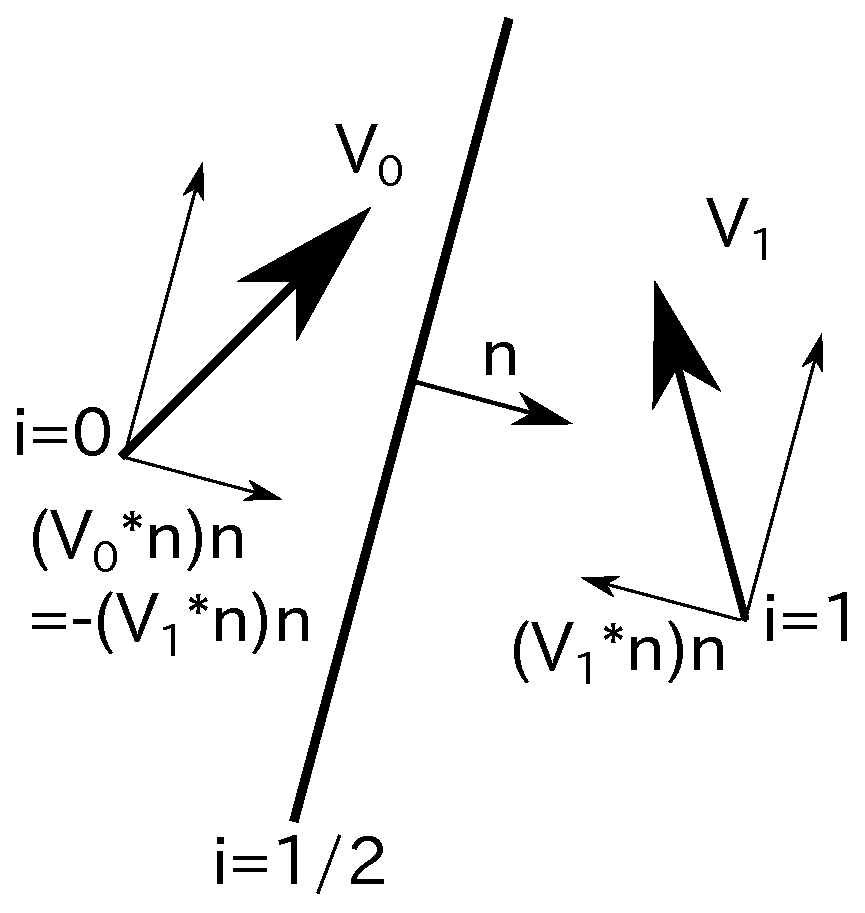
\includegraphics[width=.5\textwidth]{tutorial_img/slip_wall.eps}
%\end{center}
%よって、セル(1,j)での速度を$V_1$とすると、セル(0,j)での速度$V_0$は、境界(1/2,j)の法線ベクトルを$n$とすると
%\begin{equation}
%V_0=V_1-2(V_1\cdot n)n
%\end{equation}
%である。
%
%本プログラムでは図で$n$で示してある壁の法線ベクトルは以下の用に決めてある。
%\begin{itemize}
%\item ブロックplaneの境界(i+1/2,j)における+i方向の法線ベクトル...vni(1:2,i,j,plane)
%\item ブロックplaneの境界(i,j+1/2)における+j方向の法線ベクトル...vnj(1:2,i,j,plane)
%\end{itemize}
%よって、プログラムは以下のように書き下される。
%\begin{verbatim}
%if(gx(plane) .eq. 1) then
%   !i=1/2
%   do j=max(    1,nys(plane)),min(nye(plane),   49)
%      w(:,     0,j,plane) = w(:,1,j,plane)
%      w(2:3,   0,j,plane) = w(2:3,1,j,plane)-2d0*vni(:,0,j,plane)&
%               *dot_product(w(2:3,1,j,plane),    vni(:,0,j,plane))
%      vhi(:, 0,j,plane)   = vhi(:, 1,j,plane) 
%
%      w(:,  -1,j,plane)   = w(:,   0,j,plane) 
%      vhi(:,-1,j,plane)   = vhi(:, 0,j,plane) 
%   end do
%end if
%\end{verbatim}
%%}}}
%\subsubsection{粘着壁}%{{{
%すべり壁では速度全てを反転させる。
%そうすればi=0とi=1の平均が0になるからである。
%
%\begin{verbatim}
%if(gx(plane) .eq. 1) then
%   !i=1/2
%   do j=max(    1,nys(plane)),min(nye(plane),   49)
%      w(:,     0,j,plane) = w(:,1,j,plane)
%      w(2:3,   0,j,plane) =-w(2:3,1,j,plane)
%      vhi(:, 0,j,plane)   = vhi(:,1,j,plane) 
%
%      w(:,  -1,j,plane)   = w(:,   0,j,plane) 
%      vhi(:,-1,j,plane)   = vhi(:, 0,j,plane) 
%   end do
%end if
%\end{verbatim}
%
%%}}}
%%}}}
%%}}}
%\newpage
%\section{デバッグに関する小技集}%{{{
%プログラムを修正した際には必ずといっていいほどバグが発生する。
%
%ここでは、デバッグに利用できるコマンドをいくつか紹介する。
%\paragraph{grepコマンド}%{{{
%grepコマンドは
%\begin{verbatim}
%grep word filename
%\end{verbatim}
%で、filenameで指定されたファイルからwordに該当する部分がないか調べるコマンドである。
%例えば、main.f90にあるinit\_geometryというサブルーチンがstoreディレクトリでどこにあるかわからない場合、
%%{{{
%\begin{verbatim}
%grep init_geometry store/*{,/*{,/*{,/*{,/*{,/*}}}}}
%\end{verbatim}
%というコマンドをうつ。ここで、シェルでは\{a,b\}という文字列はaとbに展開されるので、上記コマンドは
%\begin{verbatim}
%grep init_geometry store/* store/*/* store/*/*/* store/*/*/*/* \
%store/*/*/*/*/* store/*/*/*/*/*/*
%\end{verbatim}
%というコマンドを意味する。(\verb|\|はシェルにおいて継続行を意味する。)
%このコマンドを実行すると、
%\begin{verbatim}
%store/core/main.part_init.f90:   call init_geometry
%store/dim/2d/geometry.f90:subroutine init_geometry!{{{
%store/dim/2d/geometry.f90:end subroutine init_geometry!}}}
%store/dim/q2d/geometry.f90:subroutine init_geometry!{{{
%store/dim/q2d/geometry.f90:end subroutine init_geometry!}}}
%\end{verbatim}
%と出力されることから、init\_geometryはstore/dim/2d/geometry.f90とstore/dim/q2d/geometry.f90で定義されていることがわかる。
%
%このコマンドを使えば、使われているサブルーチンがどこで定義されているのかをすぐに探すことができる。
%%}}}
%
%\paragraph{エラーメッセージから}%{{{
%上記コマンドとエラーメッセージを合わせると、エラー発生場所がわかる。
%
%例えば、完全平衡モデルにおいて収束しないと
%\begin{verbatim}
%not converted. at cea
%\end{verbatim}
%とメッセージがでるが、これがどこで判定されているか知りたいときには
%%{{{
%\begin{verbatim}
%grep "not converted. at cea" store/*{,/*{,/*{,/*{,/*{,/*}}}}}
%\end{verbatim}
%をうてば
%\begin{verbatim}
%store/therm_lib/NASA/core/sub_chem.f90:         print *,"not converted. at cea"
%store/therm_lib/NASA/core/sub_chem.f90:         print *,"not converted. at cea_hp"
%store/therm_lib/NASA/core/sub_chem.f90:         print *,"not converted. at cea_hp"
%\end{verbatim}
%とでるので、どのような条件でこのメッセージがでているのかを知ることができる。
%%}}}
%
%\paragraph{Makefileのコンパイラスイッチ}%{{{
%使用アーキテクチャにPCを選んだ場合、Makefileの冒頭が次のようになる。
%\begin{verbatim}
%##### SELECT ARCHITECTURE#######################
%#PERSONAL COMPUTER
%arc=mod_mpi_dummy.o
%compiler=ifort -convert big_endian -openmp -fast -parallel
%#compiler=ifort -convert big_endian -fast -parallel
%#compiler=ifort -convert big_endian -check all -traceback -g
%#compiler=ifort -O1
%##### END SELECT ARCHITECTURE###################
%\end{verbatim}
%ここでcompilerで定義されているコンパイラスイッチは" -convert big\_endian"以外では" -openmp -fast -parallel"だが、これは高速化を行うため、プログラム中のどのファイルのどのラインで0割りが起こったかや、どこでどのように未定義配列領域にアクセスしたのかを出力してくれない。
%
%そこで、デバッグ時には
%\begin{verbatim}
%compiler=ifort -convert big_endian -check all -traceback -g
%\end{verbatim}
%を用いると、デバッグのための情報を出力してくれる。
%
%同様に、スーパーコンピュータでは
%\begin{verbatim}
%##### SELECT ARCHITECTURE#######################
%#SUPER COMPUTER
%arc=mod_mpi.o
%compiler=f90jxflat -Umpi -Uomp
%#compiler=f90jx -Umpi -Uomp
%#compiler=f90jx -Umpi
%#compiler=f90jx -Umpi -Uomp -xert,cvr
%##### END SELECT ARCHITECTURE###################
%\end{verbatim}
%となっているが
%\begin{verbatim}
%compiler=f90jx -Umpi -Uomp -O0 -Knoparallel
%\end{verbatim}
%とすると、デバッグを行いやすくなる。
%%}}}
%%}}}
%\newpage
%
%%details
%\part{各機能の説明}
%\newpage
%\section{ライブラリ生成アルゴリズムについて}%{{{
%本プログラムは基本的に「ライブラリ生成プログラム」となる。
%よって、各種パラメータ設定ファイルに加えて、流体計算の場合は"condition.f90"というファイルで直接初期条件と境界条件を設定しなければならない。これらのファイルは"raw"というサフィックス付きでディレクトリにコピーされる。
%
%コンパイルはコピーされたディレクトリ内(checkout or checkout\_chem)のファイルのみが使用される。よって、そのディレクトリをどこか別のディレクトリにもっていっても、正常に動作する。store内のファイルがコンパイル時に使われることはない。
%
%GUIインターフェースであるGUI.pyは、checkout.pyを動かすためのinputファイル(checkout.inp, checkout\_model.inp, checkout\_chem.inp)を生成し、checkout.pyを実行するプログラムであり、主動作はGUI.pyを用いた場合でも多くをcheckout.pyが受け持つ。
%
%checkout.pyはinputファイルに基づき、各種ライブラリを生成するプログラムである。基本的にライブラリの生成は、該当ファイルをディレクトリからコピーすることによって行い、ある特定のファイルを除いてはfortranソースファイル自体をcheckout.pyが編集することはない。コピーされるファイルは全て"store"のサブディレクトリ内に入っており、checkout.pyまたはユーザーによって編集が加えられるファイルには".raw."というサフィックスがつけられている。なお、checkout.py内でそのソースファイルの編集が終了する、つまりそれ以上ユーザーによる編集が不必要になったファイルからは自動的に".raw."サフィックスが取り除かれ、そのままコンパイルにかけられるようになる。
%\subsection{ディレクトリ構造}
%基本的に類似する機能を持つファイルがまとめられている。例えばオイラー陽解法とLU-SGS法は"time\_scheme"ディレクトリ内に"euler","lu-sgs"としてそれぞれ格納されている。また化学計算と流体計算は基本的に同一ライブラリを用いることになっている。以下、全てのディレクトリについて説明を行う。
%%}}}
%\newpage
%\section{流体コード}\label{流体コード}%{{{
%checkout.inpを記入し、checkout.pyを起動すると生成される。
%実処理はcheckout.pyから呼び出された"store/checkout/checkout\_flow.py"によって生成される。生成されたファイルは"checkout"ディレクトリ内に生成される。
%\subsection{自動生成ファイル}%{{{
%流体コードで自動生成されるファイルは、checkout.pyで選択されたディレクトリ内にある"部分的なファイル"をつなげることで生成される。自動生成されるファイル及びその"部分的なファイル"は以下のとおりである。
%\begin{itemize}
%\item main.f90...主プログラムがかかれたソースとなる。主ループもここで回される。以下の順にファイルの内容が追記されていく。
%\begin{itemize}
%\item main.top.f90..."program main"からモジュールのインポートまで。
%\item main.head.f90...共通して利用する変数の定義。
%\item main.variable.f90...それぞれのスキームで特有に利用される変数の定義。
%\item main.part\_init.f90...変数の初期化。グリッドの読み込みやそのバイナリファイルの生成や幾何ヤコビアンの生成、熱力学ライブラリが必要とされる場合にはその初期化も行われる。
%\item main.body.raw.f90...初期化。restart.binがある場合はそれを用い、ない場合は初期化サブルーチンを用いて初期化を行う。また主ループを回す変数も初期化される。part\_primitiveという文字列がファイル内に記されており、後述する文字列に置き換えられる。主ループの開始まで記述してある。
%\item main.main.raw.f90, main.main.point\_implicit.f90...
%主ループ内部を記述しており、時間スキームのディレクトリ内に格納されている。
%part\_point\_implicit, part\_primitive, part\_mainという文字列がファイル内に記されており、それぞれ以下の文字列に置き換えられる
%part\_point\_implicitに文字列が存在する場合main.main.point\_implicit.f90、存在しない場合main.main.raw.f90が使われる。
%なお、point implicitなスキームを受け付けない時間積分法(ex.Dual Time Step)にはmain.main.point\_implicit.f90は存在せず、無理やり使おうとする場合コンパイルエラーが起きる。
%\begin{itemize}
%\item part\_point\_implicit...point implicitに計算される部分がここに入る。現状、化学生成項の時間積分を進めるサブルーチンがここに入りうる。main.part\_point\_implicit.f90にかかれた文字列に置き換えられる。
%\item main.part\_primitive.f90...時間刻みの計算やデータアウトプット前にすべき処理、具体的には基本量の計算及び境界条件の設定をするサブルーチンがここに入る。main.part\_primitive.f90にかかれた文字列に置き換えられる。
%\item main.part\_main.f90...高次精度化や対流項及び拡散項の計算、時間積分に必要な場合にはそれらの保存量ヤコビアンが計算される。main.part\_main.f90にかかれた文字列に置き換えられる。
%\end{itemize}
%\item main.foot.f90...主ループの終了及びMPI関数の終了処理、"end program main"を記述してある。
%\end{itemize}
%\item Makefile...Makefile. 以下の順にファイルの内容が追記されていく。
%\begin{itemize}
%\item Makefile.head...コンパイラに何を使うのか定義する。アーキテクチャ(PCかスーパーコンピュータ)によって変更される。
%\item Makefile.var ...各種変数の定義
%\item Makefile.main...各オブジェクトファイル作成ルール
%\item Makefile.foot...プログラムの最終的なコンパイル部分及びcleanの定義
%\end{itemize}
%\item control.raw.inp...cflの定義やファイル出力間隔の定義など。使用する場合、MUSCLのパラメータもここで入力される。control.part.inpに記された内容が入力される。
%\end{itemize}
%%}}}
%\subsection{store/core}%{{{
%どのような場合にも使用されるファイルがまとめられてある。上記自動生成ファイルのための各種ファイルの他、以下のファイルが存在する。
%\begin{itemize}
%\item check\_convergence.f90...収束判定及び途中経過ファイル,restartファイルの生成を行っている。
%\item init.vi...vim用初期化ファイル。これを読み込むと、RUNコマンドで./mainを走らせることができる。
%\item inout.f90...restartファイル読み書きや途中経過ファイル書き込み。
%\item n\_grid.raw.f90...重要なパラメータの定義。以下の文字列はcheckout.pyで置き換えられる。
%\begin{itemize}
%\item NPLANE...multi-blockでblockの数。muti-blockでない場合1.
%\item NumI...それぞれの面でのi方向セル数
%\item NumJ...それぞれの面でのj方向セル数
%\item NIMAX...i方向セル数最大値
%\item NJMAX...j方向セル数最大値
%\item NumY...rhoの数.ex)理想気体:1, flame sheet,完全平衡モデル:2, 素反応モデル:化学種数
%\item NV...拡散で空間微分をとるべき次元数.flame sheetで3,完全平衡モデルで化学種数.
%\item GridFileName...plot3dで記述されたグリッドファイルの場所.
%\end{itemize}
%また以下の文字列はICやBCの設定に使える。
%\begin{itemize}
%\item dimq ... q(後述)の次元
%\item dimw ... w(後述)の次元
%\item indxg ... wに於ける比熱比のインデックス
%\item indxht ... wに於ける質量あたり全エンタルピー(J/kg)のインデックス
%\item indxR ... wに於ける質量あたり気体定数(J/kg/K)のインデックス
%\item indxMu ... wに於ける粘性係数(Pa*s)のインデックス
%\end{itemize}
%\item prmtr.f90...piやモルあたりの気体定数"R\_uni"の定義.
%\item read\_control.f90...control.inpの読み込み.全計算に共通する部分に限る。
%\item scheme.f90...流束項評価サブルーチン。現在はSLAUのみ。
%\item variable.f90...一般的に使われる変数がまとめられてある。
%\begin{itemize}
%\item q ... 保存量.
%\begin{itemize}
%\item インデックス1からnY : それぞれの気体グループ(理想気体なら全化学種、flame sheetか完全平衡モデルなら燃料と酸化剤、素反応モデルならそれぞれの化学種)の密度(kg/m\^3)
%\item インデックスnY+1 : x方向運動量(kg*m/s)
%\item インデックスnY+2 : y方向運動量(kg*m/s)
%\item インデックスnY+3 : 全エネルギー(J/m\^3)
%\end{itemize}
%\item qp ... 前ステップのq
%\item qpp ... 全ステップのqp
%\item w ... 基本量
%\begin{itemize}
%\item インデックス1 : 全化学種の密度の和(kg/m\^3).
%\item インデックス2 : x方向速度(m/s).
%\item インデックス3 : y方向速度(m/s).
%\item インデックス4 : 圧力(Pa)
%\item インデックス5 ... nY+4 : それぞれの気体グループの質量分率
%\item インデックスnY+5(=indxg @n\_grid.f90) : 比熱比
%\item インデックスnY+6(=indxht@n\_grid.f90) : 全エンタルピー(J/kg)
%\item インデックスnY+7(=indxR @n\_grid.f90) : 気体定数(J/kg/K)
%\item インデックスnY+8(=indxMu@n\_grid.f90) : 粘性係数(Pa*s)
%\end{itemize}
%\item vhi ...それぞれの気体グループの生成熱を含む内部エンタルピー(J/kg)
%\item wHli,wHri, wHlj, wHrj ... 高次精度化で予測されたw( ex. MUSCL).'l'は'left'、'r'は'right'、'i'はi方向に+1/2を足した位置、'j'はj方向に1/2を足した位置。例えば、wHli(:,2,3)は$w_{2+\frac 1 2,3}$の左側の値を表す。
%\item TGi, TGj ... それぞれi方向j方向の流束項TG. TGの定義については嶋田テキストのSection 9参照. 
%これらの値も1/2だけセル中心からずれた場所の値であり、ずれ方はwHと同じ。
%\item TGvi, TGvj ... 粘性項.
%\item Vol ... 軸対称問題ではそれぞれのセルの体積、二次元問題では面積。
%\item dsi, dsj ... i方向j方向にそれぞれ垂直なセル辺の長さ。軸対称問題ではさらに半径がかけられる。これもセル中心から1/2だけずれた場所の値。
%\item vni, vnj ... それぞれdsi, dsjで示された辺の直交正規ベクトル(絶対値1).向きはi,j正の向き。これもセル中心から1/2だけずれた場所の値。
%\item xh, rh ... メッシュ格子点の座標.これもセル中心から1/2だけずれた場所の値。
%\item x, r ... セル中心の座標.
%\item dt\_mat ... local time stepのそれぞれのセルでの$\Delta t$
%\item dt\_grbl ... global time stepの$\Delta t$.(スペルミスったので'r'です。)
%\end{itemize}
%\end{itemize}
%また全ての計算において、以下の値をcontrol.inpで設定する必要がある。
%\begin{itemize}
%\item Max Step Number...計算を再開してからの最大ステップ数.
%\item convergent RMS...収束とするエネルギー残渣.
%\item CFL Number...CourantFriedrichsLewy数.
%\item File Output Period...ファイル出力周期.
%\end{itemize}
%%}}}
%\subsection{store/architecture}%{{{
%アーキテクチャ依存のサブルーチン.
%サブディレクトリはPCとSCでそれぞれPCとスーパーコンピュータに関するファイルがある.
%
%SCにはmod\_mpi.f90、PCにはmod\_mpi\_dummy.f90が使われる。
%スーパーコンピュータの場合はgrid\_separation.inpからそれぞれのプロセッサが受け持つグリッドの範囲を計算し、変数を初期化する.
%また、自動生成されたグリッドの分割の状態は、スーパーコンピュータを選んだ際に生成されるvis\_grid.datを用い、gnuplotで
%\begin{verbatim}
%plot "vis_grid.dat" with lines
%\end{verbatim}
%のコマンドを打つことで確認することができる。
%
%どちらの場合も以下のように受け持つブロックの範囲,i方向の範囲,j方向の範囲が定義される。
%\begin{itemize}
%\item ブロックの範囲...npsからnpe
%\item ブロックplaneのi方向の範囲...nxs(plane)からnxe(plane)
%\item ブロックplaneのj方向の範囲...nys(plane)からnye(plane)
%\end{itemize}
%パソコンの場合、nps=1, npe=Nplaneである。
%
%格子ブロックで境界になっているが、ブロック間で共有されており、ユーザーが直接入力する必要のない境界がある。これを本プログラムではcut\_copro*.inp, MPIcomm*.inpを用いて記録している。*はプロセッサ番号で、パソコンでは0である。cut\_copro*.inpは同一コア間でのデータ転送で足る場合、MPIcomm*.inpは異なるコア間でのデータ転送が必要な場合に使われる。よってパソコンの場合MPIcomm*.inpは出力されない。
%
%\subsubsection{PCでのMPIダミー関数の定義について}
%PCの場合はMPI関数のダミー関数を入れている。\textbf{このダミー関数は完全ではない。}つまり、例えばMPI\_Reduceの定義は
%\begin{verbatim}
%subroutine MPI_Reduce(tmpt, tmp, te, MPI_DOUBLE_PRECISION, MPI_SUM, te2, MPI_COMM_WORLD, ierr)
%    double precision tmpt, tmp
%    integer te1, MPI_DOUBLE_PRECISION, MPI_SUM, te2, MPI_COMM_WORLD, ierr
%    tmp=tmpt
%end subroutine MPI_Reduce
%\end{verbatim}
%となっており、これではMPI\_INTEGERに対応できない。
%MPI関数を使った変更をプログラムに施す際にはmod\_mpi\_dummy.f90で行われているダミー関数の定義を参照すること。
%
%\subsubsection{スーパーコンピュータ用ユーティリティについて}
%スーパーコンピュータ用にいくつかのユーティリティプログラムが用意されている。
%\paragraph{プロセッサへのグリッド割当について}
%\begin{itemize}
%\item generate\_proc\_grid.py...グリッド分割用ライブラリ。
%基本的には全てのプロセッサが持つグリッドができるだけ均等になるよう分割するが、split\_ratio.pyが存在するとき、そのsplit\_ratio.ratio(plane,cind)を用いて寄せることも可能である。
%\item trim\_balance.py...それぞれのプロセッサの計算負荷を可視化するためのプログラム。
%\end{itemize}
%
%\paragraph{ジョブキューの投入・確認・削除}
%基本的にlargeシステムで実行すること。
%\begin{itemize}
%\item mpirun.sh...\verb|sh mpirun.sh|でジョブキュー投入を行える。check\_and\_throw.pl及びStepJob.pyは内部的にmpirun.shをよんでいる。
%\item check.pl...\verb|perl check.pl|でジョブの動作状況(QUEUED, RUNNING, EXISTING)と現在出力されている最新のファイル名を一秒おきに出力する。
%\item check\_and\_throw.pl...\verb|perl check_and_throw.pl|でcheck.plの動作を行った上、全てのジョブが終了している場合、新たに\verb|sh mpirun.sh|を実行する。
%これを用いると、600秒に限られたデバッグジョブにおいて、ジョブが終わった瞬間に新しいジョブ投げることができるので、半永久的にデバッグジョブを走らせることができる。
%よって、使いっぱなしになると確実にスーパーコンピュータ利用禁止となり卒業できなくなるので、程度を考えて利用すること。
%経験上一時間程度なら怒られない。
%\item StepJob.py...\verb|python StepJob.py|で、ステップジョブを投げられるだけ投げる。つまり、実行時にステップジョブが19投げられている場合、50まで投げられるので、31回\verb|sh mpirun.sh|が実行される。これをcronと組み合わせ、
%\begin{verbatim}
%0 0,6,12,18 * * * cd /large/y/y535/2dcfd/share_code; python StepJob.py
%\end{verbatim}
%のようにしておけば、一々ターミナルを開きスーパーコンピュータにログインすることなしに、自動的に6時間おきに最大数までジョブを予約することができる。また、cronの実行結果はメールで送られるので、現在のステップ数を6時間おきにメールで知ることが可能になる。
%
%cronを利用する際の注意点として、cronはサーバー毎に設定できるらしく、同じmaja.jss.jaxa.jpでもmaja0.jss.jaxa.jp, maja1.jss.jaxa.jpが存在する.よって、crontabを編集する際には、maja0.jss.jaxa.jpなど明示的にどのサーバーを用いるのかを示してログインしなければならない。
%\item qdel.pl...\verb|perl qdel.pl|でqdelコマンドを予約している全てのジョブに投げる、つまり予約している全てのジョブをキャンセルできる。
%実行中のジョブも強制終了させる。
%プログラムが落ちた際や、間違った境界条件を使用していたことに気づいた際に用いる。
%\end{itemize}
%
%これらの中で、check.pl, check\_and\_throw.pl, StepJob.py, qdel.plはファイル中にユーザー名を書き込む必要がある。
%"y535"と書いてある部分を自分のユーザー名に置き換えること。
%
%\paragraph{データファイルの転送コマンド}
%\begin{itemize}
%\item \verb|make remove| on SC...スーパーコンピュータ上で打つと、標準入力および標準出力、result内の全ての結果を削除する。restart.binは残す。
%\item \verb|make tar| on SC...スーパーコンピュータ上で打つと、RMS.dat, geometry.bin, result/*.binをresult.tar.gzファイルに圧縮する。
%\item \verb|make pull| on postprocess...postprocessディレクトリにおいて、Makefileの変数remoteにresult.tar.gzが存在するディレクトリを指定すると、このコマンドでそのresult.tar.gzをダウンロードし解凍する。
%\end{itemize}
%%}}}
%\subsection{store/dim}%{{{
%軸対称流か二次元流かを選ぶものである。サブディレクトリは2dとq2dで、それぞれ以下のファイルが含まれている。
%\begin{itemize}
%\item store/dim/2d...geometry.f90とinit\_Sq.f90
%\item store/dim/q2d...geometry.f90とSq.f90
%\end{itemize}
%Sqは軸対称流のとき式変形の際ソース項に出てくる値を定義しており、二次元流では0である。init\_Sq.f90とSq.f90はそれぞれSqに関する処理を行っている。
%geometry.f90にはplot3dで記述されたグリッドファイルの読み込み及び可視化用バイナリファイルの生成、幾何ヤコビアンやセルの面積を計算するルーチンがまとめられている。
%%}}}
%\subsection{store/high\_order}%{{{
%高次精度化を行うルーチンである。サブディレクトリはmusclとupwindであり、それぞれMUSCLスキームと風上差分が入っている。
%MUSCLを用いる場合、以下の項目をcontrol.inpで設定する必要がある。
%\begin{itemize}
%\item MUSCL ON(1)/OFF(0)...MUSCLのon/off切り替え。1でon, 0でoff.その他の値は受け付けない。
%\item MUSCL Precision Order...MUSCLのオーダー調整。2と3のみ受けつけ、2の場合は$\kappa =-1$, 3の場合は$\kappa=\frac 1 3$にMUSCLのパラメータが設定される。
%\end{itemize}
%%}}}
%\subsection{store/time\_step}%{{{
%global time stepまたはlocal time stepが設定される。ファイルはset\_dt.f90。またこのどちらかを選ぶことにより、checkout.pyのDT\_GLOBAL\_LOCALがdt\_mat(i,j,plane)またはdt\_grblが設定され、時間積分スキームの該当する部分で置き換えられる。
%%}}}
%\subsection{store/time\_scheme}%{{{
%時間スキームの選択。main.main.raw.f90やmain.main.point\_implicit.f90,時間積分サブルーチン(time\_...f90)が入っており、主ループ(時間積分ループ)の中身を定義する。
%\begin{itemize}
%\item euler...オイラー陽解法.
%\item RK2...ルンゲ=クッタ2次精度.
%\item LU-SGS...LU-SGSで実装したオイラー陰解法.上記の他sch\_lusgs.f90, var\_lusgs.f90でLU-SGS法を行う。
%\item NR...Newton-Raphson法.同様にLU-SGS法を使う.後述するパラメータを用いる.上記の他sch\_NR.f90, var\_NR.f90でLU-SGS法を行う。
%\item precon...前処理法を用いたNewton-Raphson法.同様にLU-SGS法を使う.上記の他sch\_precon.f90, var\_precon.f90でLU-SGS法を行う。
%仮時間ステップにも前処理行列をかけている.後述するパラメータを用いる.
%\item dual...Dual Time Step.同様にLU-SGS法を使う.後述するパラメータを用いる.上記の他sch\_dual.f90, var\_dual.f90でLU-SGS法を行う。
%\item preconLU-SGS...前処理法をオイラー陰解法(LU-SGS)で実装している。上記の他sch\_precon.f90, var\_precon.f90でLU-SGS法を行う。
%\end{itemize}
%なお、LU-SGSからpreconLU-SGSには"2d"と"q2d"というディレクトリがそれぞれあるが、それぞれ二次元流、軸対称流のコードが収められている。
%
%\paragraph{NR,precon,dualで用いられるパラメータについて}%{{{
%これらのスキームでは以下のパラメータをcontrol.inpで定義する。ただし、$\omega$は内部反復の緩和係数である。
%\begin{itemize}
%\item InternalLoop CFL tau...疑似時間ステップのcfl数
%\item InternalLoop Omega Max...最大緩和係数。以下$\omega_{\max}$とする。
%\item InternalLoop Omega Min...最小緩和係数.これを割り込む$\omega$が設定されると、計算を中止する。
%\item InternalLoop Dqrate Max...各気体グループの密度の内部反復あたり変化割合の最大値.以下$Dq_{\max}$とする。
%\item InternalLoop ResRateWarn...内部反復が収束していないことを標準出力に投げる最小エネルギー残渣比
%\item InternalLoop ResRateErr...計算を中止する最小エネルギー残渣比
%\item InternalLoop OutOmega...ファイルinternal\_res.datに緩和係数$\omega$の履歴を出すか。
%\item InternalLoop Max Number...内部ループ数(固定)
%\end{itemize}
%これらのスキームの内部ループで、保存量$q$は緩和係数$\omega$をかけられた$\Delta q$により更新される。$\omega$は以下のように定義される。
%\begin{equation}
%\omega = \min(\omega_{\max} ,\frac{Dq_{\max}\rho_i}{\Delta \rho_i})
%\end{equation}
%ただし$i=1...$nYである。これにより、$\rho_i$の一内部反復での変化は$Dq_{\max}$以下に抑えられる。
%この定義であると、$\omega$が小さくなりすぎることがある。それを補足するのが"最小緩和係数"のパラメータである。
%
%内部ループの発散は'InternalLoop Omega Min', 'InternalLoop ResRateWarn', 'InternalLoop ResRateErr'で補足されることとなる。ここでエネルギー残渣比は(最後の内部反復でのエネルギー残渣)/(最初の内部反復でのエネルギー残渣)と定義している。なお、NR, precon, dualの時間スキームでは、基本コンセプトは"内部反復が収束"することに基づいているので、エネルギー残渣比が十分小さくならない場合はコンセプト自体が崩壊している。よって、その場合これらのスキームは使うべきではない。(これを見落としている研究は大変多く、私は悲しい。)
%
%\subparagraph{パラメータ調整方法}
%パラメータ調整には"internal\_res.dat"が使える。これは"InternalLoop OutOmega"を"true"にセットすることで得られる。
%(このファイル出力は時間がかかるので、本計算のときには効率向上のため"false"にすべき。)
%このファイルには1列目に内部反復数、2列目にDqrateにより計算された$\omega$($\omega_{\max}$で修正する前)、3列目にエネルギー残渣比が記録されている。
%以下にこれらの出力を使ってパラメータを調節する手段の一つを記す。
%\begin{itemize}
%\item \textbf{'InternalLoop Max Number'を増やす}...内部反復数が小さいことが原因で、エネルギー残渣比が指数的に減少しているのに'InternalLoop ResRateErr'に達していないとき。
%\item \textbf{'InternalLoop Max Number'を減らす}...'InternalLoop Max Number'に比べ遥かに少ない内部反復数で'InternalLoop ResRateErr'に達しているとき。
%\item \textbf{'InternalLoop Omega Max'を増やす}...下記の目安に比べ内部反復の収束が遥かに遅く、$\omega_{\max}$により$\omega$が主に決まっているとき。
%\item \textbf{'InternalLoop Omega Max'を減らす}...Dqrateにより決定された$\omega$('internal\_res.dat'の第二列目に記録された$\omega$)が指数的に増加せず、一回目の内部反復の$\omega$が$\omega _{\max}$により決定されている場合。
%この状況は$\omega\Delta q$があまりにも大きすぎて、一回目の内部反復における$q$の推測値が悪くなりすぎ、そのためその後のステップで正しい値に修正できなくなった場合に起こる。
%\item \textbf{'InternalLoop Dqrate Max'を増やす}...
%内部反復の収束が遅く、$\omega$がDqrateによって主に決定されている場合。
%\item \textbf{'InternalLoop Dqrate Max'を減らす}...
%$\omega$が指数的に増加せず、一回目の内部反復でDqrateにより$\omega$が決定されている場合。
%この状況も$\omega\Delta q$があまりにも大きすぎて、一回目の内部反復における$q$の推測値が悪くなりすぎ、そのためその後のステップで正しい値に修正できなくなった場合に起こる。
%\end{itemize}
%これらの手段は理論的なものではなく、私の経験によるものである。よって間違っている可能性もある。他の方法も試してください。
%
%\subparagraph{パラメータの目安}
%\begin{itemize}
%\item \textbf{0.1 @ Omega Max}...もしこれで動く場合、0.8や0.9も可能な場合もある。Dual Time Stepでは0.01を使わざるを得なかった場合もある。
%\item \textbf{0.001 @ Omega Min}...この値を下回り正しい解を出した計算に出会ったことはない。このパラメータは固定すべきであると思う。
%\item \textbf{0.01 @ Dqrate Max}...現実問題このパラメータは多分子流にのみ使われうる。Dual Time Stepでは0.001を使わざるを得なかった場合もある。経験上0.1は大きすぎる。
%\item \textbf{1.e-5 @ ResRateWarn, 1.e-3 @ ResRateErr}...経験上、エネルギー残渣比は3オーダーは下げなければ正しい解を出さない。よって1e-3は固定すべきだと考える。ResRateWarnは警告メッセージを出すだけであるので、好みの値を用いてよい。
%\item \textbf{60 @ Max Number}...理想気体では経験上20で十分。多分子流をDual Time Stepで解いたとき、100必要だった場合もあった。
%\end{itemize}
%%}}}
%
%\hspace{1em}
%
%なお、経験上precon, preconLU-SGSについては、経験上"直交格子"かつ"非燃焼流"の場合は大変うまく働くが、そのどちらかが満たされないとあまりうまく動かない。
%また、dualについてはNR以上の性能を出した経験が一度もない。
%注意すること。
%%}}}
%\subsection{store/viscosity}%{{{
%non-viscousとviscousというディレクトリがあり、viscousにはその中にwith-nVとno-nV、さらにそれぞれに"2d"と"q2d"というディレクトリが収められている。
%non-viscousが非粘性流、viscousが粘性流である。
%2dとq2dの違いはtime\_schemeと同じ。
%
%with-nVとno-nVについて、化学モデルには"単純に$\rho_i$の空間微分でエンタルピー拡散を扱えるもの"とそうでないものがあり、それぞれがwith-nVとno-nVに対応している。
%with-nVの場合、"Yv"という"質量拡散によるエンタルピー拡散を考える際考慮しなければならない気体グループの質量分率"が熱力学ライブラリから生成される。
%例えば、一段総括反応の場合、化学組成は"反応物としての"燃料と酸化剤の質量のみを追いかければいいが、質量拡散によるエンタルピー拡散を計算する場合"生成物としての"燃料、酸化剤、生成物それぞれの質量分率を計算せねばならず、with-nVが使用される。
%
%ファイルはsch\_viscous.f90である。プラントル数Prとシュミット数Scはここで名前付き定数として共に1に定義してあるので、条件を変えたい場合はここを変更するとよい。
%%}}}
%\subsection{store/therm\_lib}%{{{
%therm\_lib内には必ずthermal\_mode.f90が入っており、set\_thermo\_propというサブルーチンにより、前ステップに計算された
%\begin{quotation}
%圧力、気体定数、保存量
%\end{quotation}
%から
%\begin{quotation}
%温度の推定値、質量あたり内部エネルギー、各気体グループの質量分率
%\end{quotation}
%を計算し、そこから現ステップでの
%\begin{quotation}
%圧力、比熱比、質量あたり全エンタルピー、粘性係数、気体定数、各化学種のエンタルピーvhi、各化学種の修正生成熱DHi
%\end{quotation}
%を計算する。
%また、viscosityの節でも述べたとおり、一部熱力学ライブラリではエンタルピー拡散の計算のためにYvも計算する。
%(圧縮性流体ではエネルギー保存であるためエンタルピーは圧力依存となる。圧力は温度で変わり、温度は熱力学ライブラリで変わるため、全エンタルピーも基本量としている。)
%これら出力結果は基本量wの配列に格納される。
%
%化学ライブラリには大きくわけて理想気体,NASAデータベースを用いるもの,chemkinファイルを用いるものにわけられ、それぞれディレクトリideal,NASA,chemkinに対応する。
%NASAデータベースを用いる計算は凍結流、一段総括反応、完全平衡モデルがつかえ、
%chemkinファイルを用いる計算は凍結流、素反応モデルが使える。
%
%\paragraph{vhiとDHiの定義}%{{{
%それぞれのライブラリ詳細の説明を行う前に、vhiとDHiの説明をする。
%
%vhiはエンタルピー拡散の計算に使われ、次元はnV(Yvの次元と同じ.Yvを使わない場合はnY)である。
%それぞれの気体グループの生成エネルギーを含む単位質量あたりの内部エンタルピーである。
%拡散の計算に使われるため、vhiに関しては境界での値が必要となる。よって、適切な境界条件を設定しなければならない。
%
%DHiは修正生成熱であり、陰解法や前処理法に用いる流束の保存量でのヤコビアンを求めると出てくる。定義としては以下のとおり。
%\begin{equation}
%DHi_i=\kappa R_i T-(\kappa-1)vhi_i
%\end{equation}
%ただし、$\kappa$は混合ガス全体の平均比熱比、$R_i$はその気体グループの質量あたりの気体定数(=(一般気体定数)/(平均分子量)).
%
%$DHi_i$は理想気体では0であるが、実在気体では有限の値を持つ。また、陰解法を許さない熱力学モデルでは、これは0にセットされている。
%%}}}
%
%\subsubsection{store/therm\_lib/ideal}%{{{
%\begin{center}
%\begin{tabular}{cccc}\hline
%特有モジュール & nY & nV & with-nV or no-nV\\\hline \hline
%gas            &  1 &  1 & no-nV\\
%\hline
%\end{tabular}
%\end{center}
%
%\begin{center}
%\begin{tabular}{c||c}\hline
%使用可能時間ステップ & global, local\\
%使用可能時間スキーム & euler, RK2, LU-SGS, NR, precon, dual, preconLU-SGS\\
%\hline
%\end{tabular}
%\end{center}
%
%理想気体。ファイルはthermal\_model.f90のみである。粘性係数は動粘性係数一定の場合にのみ現在対応している。質量あたり気体定数R\_gas、比熱比kappa\_gas、動粘性係数nu\_gasは"module gas"をインポートすれば使用可能であり、checkout.pyでそれぞれ1.4,287,1.6e-5に定義されるが、thermal\_model.f90の該当部分を直接編集すれば任意の値に変更可能である。境界条件設定時にはぜひ"module gas"をインポートして上記の名前付き定数を使っていただきたい。
%
%保存量、基本量やvhiは以下のように表される。ただし、$\rho,u,v,p$は密度、x,y方向速度、圧力である。
%\begin{verbatim}
%q(1)=rho
%q(2)=rho*u
%q(3)=rho*v
%q(4)=p/(kappa_gas-1d0)
%
%w(1)=rho
%w(2)=u
%w(3)=v
%w(4)=p
%w(5)=1d0
%w(indxg )=kappa_gas
%w(indxht)=kappa_gas/(kappa_gas-1d0)*p/rho+0.5d0*(u**2+v**2)
%w(indxR )=R_gas
%w(indxMu)=rho*nu_gas
%
%vhi(1)=kappa_gas/(kappa_gas-1d0)*p/rho
%DHi(1)=0d0
%\end{verbatim}
%%}}}
%\subsubsection{store/therm\_lib/NASA}\label{store/therm_lib/NASA}%{{{
%\begin{center}
%\begin{tabular}{cccc}\hline
%特有モジュール               & nY &            nV & with-nV or no-nV\\\hline \hline
%const\_chem, chem, chem\_var &  2 &  モデルによる & with-nV\\
%\hline
%\end{tabular}
%\end{center}
%
%%共通事項{{{
%このモデルを選択する際にはchem.inpが存在しなければならない。
%
%NASA-CEA用に公開されたデータベースを用いた熱力学モデル集。凍結流と一段総括反応(flame sheet)、完全平衡モデルを用意している。
%
%気体グループは2つであり、ライブラリでは一つ目に燃料、二つ目に酸化剤を当てている。
%
%全てのモデルで使用される熱力学モデルはcore内に格納されており、以下のファイルがある。
%\begin{itemize}
%\item LU.f90...LU分解で線形連立方程式を解くモジュール.完全平衡モデルで利用されている。
%\item thermo.inp...NASA-CEA内に格納されている熱力学データ.
%\item trans.inp...NASA-CEA内に格納されている熱輸送データ.
%\item func\_chem.f90...熱力学関数多項式の係数を返す関数ライブラリ.
%\item mod\_chem.raw.f90...NASAデータベースを用いた計算に必要なモジュール.(上述特有モジュール)変数後述.
%\item sub\_chem.f90...mod\_chem内の変数初期化やinputファイル読み込み、上述反応モデルの全てのコア部のサブルーチン.
%\end{itemize}
%
%\paragraph{mod\_chem.f90の変数について}%{{{
%\subparagraph{const\_chem}定数と重要な値(化学種数)を格納している.
%\begin{itemize}
%\item ne...原子種数
%\item max\_ns...最大化学種数
%\item Ru...一般気体定数(prmtr.f90と同じ値ではあるが、化学ライブラリのみで0次元を行うときのために定義している。)
%\item pst=1d5...標準状態の圧力
%\item omega=0.5d0...一段総括反応モデルで用いられる緩和係数
%\item eps=1d-9...収束計算に用いる微小量.基準値がこれ以下になればよい.
%\item initial\_eps=1d-5...完全平衡モデルで係数行列の行列式が0にならないようにそれぞれの化学種量初期値に加える微小量
%\item Y\_eps=1d-6...完全平衡モデルで使用。燃料または酸化剤の質量分率がこれ以下の場合、存在しえない原子種に関する拘束条件を計算から排除する.
%\item TSIZE=1d-11...完全平衡モデルで使用。EとHを計算する際、物質量がこれ以下の場合その分子がもつエネルギーやエンタルピーは計算しない。
%\item TTSIZE=1d-14...完全平衡モデルで使用。各原子の量に関する拘束条件を計算するとき、物質量がこれ以下の分子は計算にいれない。
%\item ns...化学種数.
%\item nt...粘性係数の計算に使われる化学種数。化学組成の計算をする際に使われる化学種の内、trans.inpに含まれる化学種の数となる。
%\end{itemize}
%
%\subparagraph{chem}計算のコアとなるデータ.
%\begin{itemize}
%\item num\_sctn...それぞれの化学種の熱力学関数多項式の区間の数.最大値6.
%\item MW...それぞれの化学種の分子量
%\item Trange...ぞれぞれの区間の始めとおわりの温度.例えば化学種iのj番目の区間はTrange(1,j,i)KからTrange(2,j,i)Kまで.
%\item co...それぞれの区間の熱力学関数の多項式の係数.例えば化学種iのj番目の区間の多項式の係数はco(1:9,j,i).
%\item SYM\_ELM...それぞれの原子種の記号。(HEやH,Oなど)
%\item SYM\_SPC...それぞれの化学種の記号。(CO2やH2Oなど)
%\item trans...輸送係数の多項式の係数。熱力学関数のcoに対応。
%\item Trange\_trans...輸送係数の区間の端の値。熱力学関数のTrangeに対応。
%\item species\_name\_trans...熱力学関数のSYM\_SPCに対応
%\item num\_sctn\_trans...熱力学関数のnum\_sctnに対応
%\item tr2th...輸送係数のインデックスを熱力学関数のインデックスの変換するもの。
%例えばH2Oのインデックスが輸送係数ではi、熱力学係数がj(このときspecies\_name\_trans(i)とSYM\_SPC(j)は共に'H2O'である。)の場合、
%tr2th(i)=jである。
%\item Ac...それぞれの化学種に含まれる原子の数.例えば原子H,C,Oのインデックスがそれぞれ1,2,3、分子H2Oのインデックスが1の場合、Ac(1,1)=2,Ac(2,1)=0,Ac(3,1)=1である。
%\end{itemize}
%
%\subparagraph{chem\_var}境界条件で使うための燃料,酸化剤のそれぞれの各種値、及びそれぞれのセルの前ステップでの化学組成の記録。
%\begin{itemize}
%\item n\_save...完全平衡モデルで使用。各セルの前ステップでの組成。これを初期値に使うことで、反復回数が減る。
%\item qf,wf...それぞれ燃料の速度が0のときの保存量、基本量。
%\item rhof,pf,Tf,Ef,Hf,MWf,kappaf,muf...それぞれ燃料の密度、圧力、温度、質量あたり内部エネルギー、質量あたり内部エンタルピー、分子量、比熱比、粘性係数
%\item Yvf,vhif...それぞれ燃料のYf,vhi
%\item b0f...完全平衡モデルで使用。燃料の単位質量あたりそれぞれの原子物質量.
%\item nf...完全平衡モデルで使用。燃料単体に完全平衡モデルを用いたときの組成
%\item nfini...燃料単体の反応前の組成
%\item nef...完全平衡モデルで使用。燃料に含まれる原子種数.
%\item elistf...完全平衡モデルで使用。燃料に含まれる原子種のインデックス.
%\item nelistf...完全平衡モデルで使用。燃料に含まれない原子種のインデックス.
%\item maskf...完全平衡モデルで使用。各化学種で、存在しうるものが1、しえないものに0が入っている。
%\item maskbf...完全平衡モデルで使用。拘束条件で、使用するものに1、しないものに0が入っている。
%\item np...一段総括反応モデルで使用。生成物の組成。
%\item of...当量でのo/f
%\end{itemize}
%また、上記には燃料のみ記してあるが、"f"を"o"に変えれば酸化剤のそれぞれを表すことになる。
%%}}}
%
%\paragraph{境界条件での入力について}%{{{
%
%境界条件での入力に関して。例えば酸化剤のみのセルで条件を入力する場合、保存量、基本量やvhiは以下のように表される。ただし、$u,v$はx,y方向速度である。
%DHiについてはset\_thermo\_propで直接入力されるため、手作業で入力されることはない。
%\begin{verbatim}
%q(1)=0d0
%q(2)=rhoo
%q(3)=rhoo*u
%q(4)=rhoo*v
%q(5)=rhoo*Eo
%
%w(1)=rhoo
%w(2)=u
%w(3)=v
%w(4)=po
%w(5)=0d0
%w(6)=1d0
%w(indxg )=kappao
%w(indxht)=Ho+0.5d0*(u**2+v**2)
%w(indxR )=R_uni/MWo
%w(indxMu)=muo
%
%vhi=vhio
%\end{verbatim}
%燃料では"o"を"f"に変える他、\verb|q(1)=rhof;q(2)=0d0;w(5)=1d0;w(6)=0d0|になる。
%%}}}
%
%\hspace{1em}
%
%以下、凍結流と一段総括反応(flame sheet)、完全平衡モデルについてそれぞれ説明する。
%%}}}
%
%\paragraph{凍結流モデル}%{{{
%\begin{center}
%\begin{tabular}{c||c}\hline
%使用可能時間ステップ & global, local\\
%使用可能時間スキーム & euler, RK2, LU-SGS, NR, precon, dual, preconLU-SGS\\
%\hline
%\end{tabular}
%\end{center}
%凍結流モデルでは、酸化剤と燃料の混合は扱うが、その反応は考えない。つまり、酸化剤と燃料は混合されたところで反応しない。よって凍結流となる。
%凍結流モデルには、GUI.pyで一段総括反応モデルを選ぶと得られるchem.inpとcontrol\_chem.raw.inpを用いる。
%control\_chem.raw.inpは適切な修正をした後に名前をcontrol\_chem.inpとし、chem.inpと共に実行ファイルがあるディレクトリ直下に入れなければならない。
%control\_chem.inpの中身は以下のようになっている。
%\begin{verbatim}
%#Control parameters for chemistry
%Oxidizer Pressure(Pa)   : 1.e5
%Oxidizer Temperature(K) : 300.
%Oxygen Composition(mole ratio):
%N2 4
%O2 1
%end
%Fuel Pressure(Pa)       : 1.e5
%Fuel Temperature(K)     : 300.
%Fuel Composition(mole ratio):
%H2 1
%end
%Products Composition(mole ratio):
%H2O 2
%end
%\end{verbatim}
%"Products Composition"以下の行は一段総括反応のときのみ使用するのでここでは説明しない。凍結流モデルにこのインプットファイルを使った場合、これらは無視される。
%
%酸化剤と燃料はそれぞれの圧力と温度、そのモル比での組成を入力する必要がある。圧力と温度はそれぞれ単位Pa,Kで入力する。
%このインプットファイルではそれぞれ1.e5、300.となっている。
%
%組成は"化学種名 モル分率"の順で一化学種に一行用いて入力し、最後の行には"end"のみの行を入力する。モル分率の和が1である必要はない。
%このインプットファイルでは、酸化剤にN2:O2=4:1の混合気体(空気)、燃料にH2純粋気体を用いることとなっている。
%
%ファイルはthermal\_model.f90のみである。メインの計算はsub\_chem.f90内のcold\_flowが行うこととなる。
%また、nV=2である.
%%}}}
%\paragraph{一段総括反応モデル}%{{{
%\begin{center}
%\begin{tabular}{c||c}\hline
%使用可能時間ステップ & global, local\\
%使用可能時間スキーム & euler, RK2, LU-SGS, NR, precon, dual, preconLU-SGS\\
%\hline
%\end{tabular}
%\end{center}
%store/therm\_lib/NASA/flame\_sheet内に格納されており、flow, mono, plotがある。
%monoとplotは0次元計算用のライブラリであり、流体計算にはflowのみが使われる。
%
%flowには自動生成ファイル用のファイル以外にはthermal\_model.f90のみが存在する。
%これは実質的にはsub\_chem.f90のflame\_sheetを呼び出すためだけのルーチンとなり、
%メインの計算はflame\_sheetが行うこととなる。
%
%一段総括反応モデルでは組成は自由エネルギーが最小になるように決まる。
%一段総括反応モデルには、GUI.pyで完全平衡モデルを選ぶと得られるchem.inpとcontrol\_chem.raw.inpを用いる。
%control\_chem.raw.inpは適切な修正をした後に名前をcontrol\_chem.inpとし、chem.inpと共に実行ファイルがあるディレクトリ直下に入れなければならない。
%control\_chem.inpの中身は例えば以下のようになっている。
%\begin{verbatim}
%#Control parameters for chemistry
%Oxidizer Pressure(Pa)   : 1.e5
%Oxidizer Temperature(K) : 300.
%Oxygen Composition(mole ratio):
%N2 4
%O2 1
%end
%Fuel Pressure(Pa)       : 1.e5
%Fuel Temperature(K)     : 300.
%Fuel Composition(mole ratio):
%H2 2
%end
%Products Composition(mole ratio):
%N2  4
%H2O 2
%end
%\end{verbatim}
%酸化剤と燃料はそれぞれの圧力と温度、そのモル比での組成を入力する必要がある。
%圧力と温度はそれぞれ単位Pa,Kで入力する。
%このインプットファイルではそれぞれ1.e5、300.となっている。
%生成物はそのモル比での組成のみ入力する。
%
%組成は"化学種名 モル分率"の順で一化学種に一行用いて入力し、最後の行には"end"のみの行を入力する。
%このインプットファイルでは、酸化剤にN2:O2=4:1の混合気体(空気)、燃料にH2純粋気体を用いることとなっている。
%モル分率の和が1である必要はないが、酸化剤、燃料、生成物の量の分母は一致させなければならない。
%つまり、このファイルで生成物の組成を"N2 2","H2O 1"としてはならない。
%このような入力を行うと、反応式の右辺と左辺の原子の数が釣り合わないことを感知し、以下のようなエラーメッセージを出す仕様となっている。
%\begin{verbatim}
%ERROR: The amount of element: H
%ERROR: does not balance between reactants and products.
%ERROR: Please modify 'control_chem.inp'.
%\end{verbatim}
%できるだけ化学反応式のそれぞれの化学種の係数をそのまま入力するようにすること。
%
%また境界条件において、燃料だけ、酸化剤だけではなく、その間、または入力した以外の圧力、温度を持つ組成を欲しい場合がある。
%その際は、thermal\_model.f90にある\verb|YPT2w(Yf,p,T,wt,vhit)|(入力=Yf:燃料質量分率,p:圧力,T:温度)(出力=wt:速度0での基本量w,vhit:vhi)を使う.
%これ以外の境界条件が欲しい場合(ほとんどの研究ではこのような場合に出くわす)は自分で作成すること。
%
%また、nV=3であり、Yv(1),Yv(2),Yv(3)にはそれぞれ反応後の燃料、酸化剤、生成物の質量分率が入る。
%%}}}
%\paragraph{完全平衡モデル}%{{{
%\begin{center}
%\begin{tabular}{c||c}\hline
%使用可能時間ステップ & global, local\\
%使用可能時間スキーム & euler, RK2, LU-SGS, NR, precon, dual, preconLU-SGS\\
%\hline
%\end{tabular}
%\end{center}
%store/therm\_lib/NASA/cea内に格納されており、このディレクトリにはflow, mono, plot, reductionがある。
%mono, plot, reductionは0次元計算用のライブラリであり、流体計算にはflowのみが使われる。
%
%flowには自動生成ファイル用のファイル以外にはthermal\_model.f90のみが存在する。
%これは実質的にはsub\_chem.f90のceaを呼び出すためだけのルーチンとなり、
%メインの計算はceaが行うこととなる。
%
%完全平衡モデルでは酸化剤と燃料はどちらかがなくなるまで反応を行う。組成は酸化剤と燃料の相対的な量で決まる。
%完全平衡モデルには、GUI.pyで一段総括反応モデル(flame sheet model)を選ぶと得られるchem.inpとcontrol\_chem.raw.inpを用いる。
%control\_chem.raw.inpは適切な修正をした後に名前をcontrol\_chem.inpとし、chem.inpと共に実行ファイルがあるディレクトリ直下に入れなければならない。
%control\_chem.inpの中身は例えば以下のようになっている。
%\begin{verbatim}
%#Control parameters for chemistry
%Oxidizer Pressure(Pa)   : 1.e5
%Oxidizer Temperature(K) : 300.
%Oxygen Composition(mole ratio):
%N2 4
%O2 1
%end
%Fuel Pressure(Pa)       : 1.e5
%Fuel Temperature(K)     : 300.
%Fuel Composition(mole ratio):
%H2 2
%end
%Products Composition(mole ratio):
%N2  4
%H2O 2
%\end{verbatim}
%酸化剤と燃料はそれぞれの圧力と温度、そのモル比での組成を入力する必要がある。
%圧力と温度はそれぞれ単位Pa,Kで入力する。
%このインプットファイルではそれぞれ1.e5、300.となっている。
%また、一段総括反応モデルと同様に、生成物の組成も定義する必要がある。
%純粋な完全平衡モデルではこの条件は必要ではない。生成物の組成は自由エネルギー最小という条件から求まるためである。
%本プログラムでこの量を定義しているのは、必要以上に計算負荷があがることを防ぐために、
%ほとんど酸化剤の場合やほとんど燃料の場合には一段総括反応を使用することにしているためである。
%この"ほとんど"を定義するために、許容温度誤差(K)と切り替えパラメータをチェックする周期をcontrol.inpに定義する必要がある。
%完全平衡モデルを用いる際には、以下をcontrol.inpで定義する必要がある。
%\begin{verbatim}
%#FOR CFH
%Temp. Diff Limit(K)     : 1.e-3
%cfh check freq.         : 500
%\end{verbatim}
%cfhとは"cea-flame sheet hybrid scheme"の略で、"cea"は完全平衡モデル、"flame sheet"は一段総括反応モデルを表している。
%この入力例では500ステップ毎にどのくらい"ほとんど"燃料または酸素であれば温度の誤差が$10^{-3}$K以下になるかを計算し、
%他のステップではその閾値を用いて完全平衡モデルと一段総括反応の切り替えを行っている。
%
%このモデルを使うと、計算時には以下のような文字列が標準出力に吐かれる。
%\begin{verbatim}
%step=    61633500 fs/all(%)=   84.58 Yf_cfh=  1.3E-08 Yo_cfh=  0.0E+00
%\end{verbatim}
%\begin{itemize}
%\item fs/all(\%)...全てのセルの中で、flame sheetモデルを使用している割合。この場合、全セル中85\%のセルが一段総括反応モデルを用いて計算されている。
%\item Yf\_cfh...燃料質量分率がこの値以下だった場合、セル内はほとんど酸化剤だとして、flame sheetモデルが用いられる。
%\item Yo\_cfh...酸化剤質量分率がこの値以下だった場合、セル内はほとんど燃料だとして、flame sheetモデルが用いられる。
%\end{itemize}
%
%組成は"化学種名 モル分率"の順で一化学種に一行用いて入力し、最後の行には"end"のみの行を入力する。
%このインプットファイルでは、酸化剤にN2:O2=4:1の混合気体(空気)、燃料にH2純粋気体を用いることとなっている。
%
%計算のアルゴリズムには基本的にNASA-CEAと同じものが使われる。
%特に、緩和係数は一段総括反応モデルのような固定ではなく、様々なパラメータの増減をみた値となっている。
%また、ほぼ燃料または酸化剤の場合、係数行列に逆行列がなくなる場合がある。
%これは、存在しない原子の量に関する拘束条件が、収束近くなると係数がすべて0になるからである。
%よって、これらのときにその拘束条件を削除するアルゴリズムを実装しており、その際、nef,elistf,nelistf,maskf,maskbfなどの配列が使われる。
%また、複数の原子がある同一の化学種のみに含まれるような平衡状態が解の場合、それらの原子の量に関する拘束条件が数学的に同値となり、係数行列のランクが落ちる。
%この場合、NASA CEAでは特殊な処理が行われるらしいが、本プログラムではこのような状態をさけるため、拘束条件に$10^{-30}$程度の微小量を加えている。
%この数は使用するモデルによって変更せねばならない可能性がある。
%
%また、nV=nsであり、Yvにはそれぞれの化学種の質量分率が入る。
%
%また、chem.inpには使用する原子種と化学種のリストが入る。よって、この化学種のリストを変更すれば、簡略化モデルとなる。この簡略化については0次元化学計算の章で言及する。
%%}}}
%%}}}
%\subsubsection{store/therm\_lib/chemkin}%{{{
%\begin{center}
%\begin{tabular}{cccc}\hline
%特有モジュール               &       nY & nV & with-nV or no-nV\\\hline \hline
%const\_chem, chem, chem\_var & 化学種数 & nY & no-nV\\
%\hline
%\end{tabular}
%\end{center}
%
%%共通事項{{{
%このモデルを選択する際にはchem.inpが存在しなければならない。
%
%"thermo all"を用いたthermo.inpを必要としない形式のchemkin.inpの使用を前提とした熱力学ライブラリである。
%凍結流と素反応モデルを用意している。
%
%気体グループは一つ一つが単一の化学種に対応する。つまり、$\rho _i$の次元は化学種数となる。
%
%全てのモデルで使用される熱力学モデルはcore内に格納されており、以下のファイルがある。
%\begin{itemize}
%\item MW.inp...それぞれの原子の名前と原子量の一覧
%\item trans.inp...NASA-CEA内に格納されている熱輸送データ.
%\item dvode.f...odepackのパッケージの一つであるdvode.fに修正を加えたもの
%\item mod\_chem.raw.f90...chem.inpを用いた計算に必要なモジュール.(上述特有モジュール)変数後述.
%\item sub\_chem.f90...mod\_chem内の変数初期化やinputファイル読み込み、上述反応モデルの全てのコア部のサブルーチン.
%NASAデータベースでのfunc\_chem.f90の内容も統一して格納している.
%\end{itemize}
%
%なお、control\_chem.inpについて、NASAデータベースを用いた場合にはモデル作成時に生成するようにしているが、
%chemkin.inpの場合、テンプレートを"control\_chem.raw.inp"を他のファイルと同じ場所に生成するようにしている。
%
%\paragraph{dvode.fに加えた修正について}%{{{
%dvode.fはOpenMPに直接用いるとエラーを起こす。これは、common文に含まれる変数がプロセッサ間で共有されてしまうからである。
%そのため、本ライブラリに含むdvode.fにはthreadprivate属性を付け加えている。
%
%また、警告メッセージを標準出力に出力すると標準出力がそれで埋め尽くされてしまうので、標準出力への警告出力も抑制してある。
%%}}}
%
%\paragraph{mod\_chem.f90の変数について}%{{{
%\subparagraph{const\_chem}定数と重要な値(化学種数)を格納している.
%\begin{itemize}
%\item erg2cal=1d0/4.184e7...ergからcalへの単位変換に用いる定数.ergの値にかけるとcalになる
%\item cal2erg=1d0/erg2cal...calからergへの単位変換に用いる定数。
%\item b2Pa=0.1d0...baryeからPaへの単位変換に用いる定数。
%\item Pa2b=1d0/b2Pa...Paからbaryeへの単位変換に用いる定数。
%\item Ru=8.3144621d7...cgs単位系での気体定数。
%\item invRc=1d0/(1.987e0)...cal/(mol*K)で表した気体定数の逆数.活性化エネルギーに対して用いる。
%\item pst=1.01325d6...単位系dyn/cm\^2での標準状態圧力
%\item logPR=-4.407418526701446...=ln(Pst/Ru)
%\item n\_eps = 1d-40...n(mol/cm\^3)に用いる微小量.初期値がこれ以下である場合、この値にして計算を回す。
%\item rtol\_user,atol\_user...それぞれユーザー定義の相対許容誤差、絶対許容誤差
%\item isColdFlow...凍結流の計算でtrue、それ以外でfalseが設定される。trueが設定されると、温度計算反復で化学種を反応物に含まれるものしか考慮しなくなる。
%\item max\_ne,ne...最大原子種数及び原子種数
%\item max\_ns,ns...最大化学種数及び化学種数
%\item max\_nr,nr...最大素反応数及び素反応数
%\item num\_reac...反応物で使われている化学種数
%\item LRW=22+9*(max\_ns+1)+2*(max\_ns+1)**2...dvode用に確保する実数型作業用配列の次元
%\item LIW=30+  (max\_ns+1)...dvode用に確保する整数型作業用配列の次元
%\item max\_recalc=50...dvodeでこの回数以上再計算を行う場合、計算を止める。(一回の計算で500回の内部反復をdvodeは行うので、500*50=25,000回の内部反復となる。)
%\end{itemize}
%
%\subparagraph{chem}計算のコアとなるデータ.
%\begin{itemize}
%\item nt...粘性係数の計算に使われる化学種数。化学組成の計算をする際に使われる化学種の内、trans.inpに含まれる化学種の数となる。
%\item ns\_tocalc...isColdFlow=.true.の場合num\_reac, isColdFlow=.false.の場合ns。
%\item SYM\_ELM...それぞれの原子種の記号。(HEやH,Oなど)
%\item SYM\_SPC...それぞれの化学種の記号。(CO2やH2Oなど)
%\item SYM\_RCT...それぞれの素反応の記号。('CH2CO+H=CH3+CO'など)
%\item ES...それぞれの化学種に含まれる原子の数.例えば原子H,C,Oのインデックスがそれぞれ1,2,3、分子H2Oのインデックスが1の場合、ES(1,1)=2,ES(2,1)=0,ES(3,1)=1である。
%\item Tthre...ぞれぞれの区間の始めとおわりの温度.例えば化学種iのj番目の区間はTthre(1,j,i)KからTthre(2,j,i)Kまで.
%\item coeff...それぞれの区間の熱力学関数の多項式の係数.例えば化学種iのj番目の区間の多項式の係数はcoeff(1:7,j,i).
%\item MWs...それぞれの化学種の分子量
%\item invMW...MWsの逆数
%\item Rstate...素反応の分類
%\begin{itemize}
%\item Rstate(1,:)...双方向反応か一方向反応か
%\begin{itemize}
%\item Rstate(1,:)=0:双方向反応('$=$'や'$<=>$'など)
%\item Rstate(1,:)=1:一方向反応('$=>$'で表される反応)
%\end{itemize}
%\item Rstate(2,:)...反応係数のモデル
%\begin{itemize}
%\item Rstate(2,:)=0:逆反応を平衡係数から求める.
%\item Rstate(2,:)=1:双方向の反応係数の係数がそれぞれ存在する(rev)
%\item Rstate(2,:)=2:Lindemann式(low)
%\item Rstate(2,:)=3:TROE式(troe)
%\item Rstate(2,:)=4:第三体が必ず存在する反応(第三体に括弧がつかない反応)で逆反応を平衡係数から求める.
%\item Rstate(2,:)=5:第三体が必ず存在する反応(第三体に括弧がつかない反応)で双方向の反応係数の係数がそれぞれ存在する.
%\end{itemize}
%\end{itemize}
%\item NumNu...右辺左辺それぞれの反応体数(素反応jが2H2O2=2H2O+O2ならNumNu(1,j)=2, NumNu(1,j)=3)
%\item IndNu...右辺左辺それぞれの反応体のインデックス
%(素反応jが2H2O2=2H2O+O2でH2O2,H2O,O2のインデックスがそれぞれ1,2,3なら、
%IndNu(1,1,j)=1; IndNu(2,1,j)=1 ;IndNu(1,2,j)=2; IndNu(2,2,j)=2; IndNu(3,2,j)=3)
%\item snu...snu(j)=NumNu(2,j)-NumNu(1,j)
%\item duplicate...chem.inpでduplicate属性がついているなら.true.、ついていないなら.false.。
%\item exist\_M...第三体を含む反応ならtrue、含まないならfalse
%\item NumM...enhance factorが設定されている場合、それを持つ化学種数(H2O/2/ O2/3/なら2)
%\item IndM...enhance factorをもつ化学種のインデックス(素反応kのenhance factorがH2O/2/ O2/3/かつH2O,O2のインデックスがそれぞれ2,3なら、IndM(1,k)=2;IndM(2,k)=3)
%\item Men...enhance factor から1を引いたもの(素反応kのenhance factorがH2O/2/ O2/3/なら、Men(1,k)=1;Men(2,k)=2)
%\item ABE...反応係数$k=AT^\beta \exp(-E/RT)$のとき、ABE(1)=$\ln A$, ABE(2)=$\beta$, ABE(3)=$E/R$.
%\item cABE...revやlowのABE
%\item TROE...troeフォームの係数. 
%TROE(1)=$a$, TROE(2)=$1/T^{***}$, TROE(3)=$1/T^{*}$, TROE(4)=$T^{**}$
%\item species\_name\_trans...熱力学関数のSYM\_SPCに対応
%\item Trange\_trans...輸送係数の区間の端の値。熱力学関数のTthreに対応。
%\item trans...輸送係数の多項式の係数。熱力学関数のcoeffに対応。
%\item num\_sctn\_trans...それぞれの化学種の輸送係数関数多項式の区間の数.
%\item tr2th...輸送係数のインデックスを熱力学関数のインデックスの変換するもの。
%例えばH2Oのインデックスが輸送係数ではi、熱力学係数がj(このときspecies\_name\_trans(i)とSYM\_SPC(j)は共に'H2O'である。)の場合、
%tr2th(i)=jである。
%\end{itemize}
%
%\subparagraph{chem\_var}境界条件で使うための燃料,酸化剤のそれぞれの各種値。
%\begin{itemize}
%\item qf,wf...それぞれ燃料の速度が0のときの保存量、基本量。
%\item rhof,pf,Tf,Ef,Hf,MWf,kappaf,muf...それぞれ燃料の密度、圧力、温度、質量あたり内部エネルギー、質量あたり内部エンタルピー、分子量、比熱比、粘性係数
%\item vrhof...qf(1:ns)
%\item vwf...wf(5:ns+4)
%\item vhif...燃料のvhi
%\item of...当量でのo/f.0次元計算のときのみ使用。
%\end{itemize}
%また、上記には燃料のみ記してあるが、"f"を"o"に変えれば酸化剤のそれぞれを表すことになる。
%%}}}
%
%\paragraph{uvhpについて}%{{{
%store/therm\_lib/chemkinにはuvhpというディレクトリがあり、uvとhpというディレクトリがその中に含まれている
%uvとhpというディレクトリにはFJ.f90が含まれており、それぞれuv一定,hp一定条件のサブルーチン群が含まれている。
%圧縮性流体の場合、保存量がuv一定であるため、自動的にuvディレクトリが使用される設定になっている。
%%}}}
%
%\paragraph{境界条件での入力について}%{{{
%境界条件での入力に関して。例えば酸化剤のみのセルで条件を入力する場合、保存量、基本量やvhiは以下のように表される。ただし、$u,v$はx,y方向速度である。
%DHiについてはset\_thermo\_propで直接入力されるため、手作業で入力されることはない。
%\begin{verbatim}
%q(:)=qo
%q(nY+1)=rhoo*u
%q(nY+2)=rhoo*v
%q(nY+3)=qo(nY+3)+0.5d0*rhoo*(u**2+v**2)
%
%w(:)=wo
%w(2)=u
%w(3)=v
%w(indxht)=wo(indxht)+0.5d0*(u**2+v**2)
%vhi=vhio
%\end{verbatim}
%燃料では"o"を"f"に変える。
%%}}}
%
%\hspace{1em}
%
%以下、凍結流と素反応モデルについてそれぞれ説明する。
%%}}}
%
%\paragraph{凍結流モデル}%{{{
%\begin{center}
%\begin{tabular}{c||c}\hline
%使用可能時間ステップ & global, local\\
%使用可能時間スキーム & euler, RK2, LU-SGS, NR, precon, dual, preconLU-SGS\\
%\hline
%\end{tabular}
%\end{center}
%store/therm\_lib/chemkin/flow/coldに格納されている。
%
%凍結流モデルでは、酸化剤と燃料の混合は扱うが、その反応は考えない。つまり、酸化剤と燃料は混合されたところで反応しない。よって凍結流となる。
%凍結流モデルを選んだ流体コードを生成すると、checkoutディレクトリにcontrol\_chem.raw.inpが生成される。
%これは適切な修正をした後に名前をcontrol\_chem.inpとし、chem.inpと共に実行ファイルがあるディレクトリ直下に入れなければならない。
%control\_chem.inpの中身は以下のようになっている。
%\begin{verbatim}
%#Control parameters for chemistry
%Oxidizer Pressure(Pa)   : 1.e5
%Oxidizer Temperature(K) : 1200.
%Oxygen Composition(mole ratio):
%O2 2
%end
%Fuel Pressure(Pa)       : 1.e5
%Fuel Temperature(K)     : 1200.
%Fuel Composition(mole ratio):
%CH4 1
%end
%Relative Torelance VODE : 1.e-8
%Absolute Torelance VODE : 1.e-20
%\end{verbatim}
%酸化剤と燃料はそれぞれの圧力と温度、そのモル比での組成を入力する必要がある。圧力と温度はそれぞれ単位Pa,Kで入力する。
%このインプットファイルではそれぞれ1.e5、1200.となっている。
%
%組成は"化学種名 モル分率"の順で一化学種に一行用いて入力し、最後の行には"end"のみの行を入力する。モル分率の和が1である必要はない。
%このインプットファイルでは、酸化剤にO2純粋気体、燃料にCH4純粋気体を用いることとなっている。
%
%また、VODEに用いる相対許容誤差と絶対許容誤差も定義しなければならない。(凍結流では実際にこの値は使われることはない。)例に載せてある値はSENKINに使われている値である。これらの値は大きくするとそれだけ計算が早くなるが、大きくしすぎると計算が破綻する(発散する)。
%
%境界条件には\verb|calc_boundary(p,T,Yf, wt,vhit)|を用いる。仕様はNASAデータベースで用いられている\verb|YPT2w(Yf,p,T,wt,vhit)|と同様である。
%
%また凍結流の計算では、化学種は反応物に含まれるものしか考慮されない。
%%}}}
%\paragraph{素反応モデル}%{{{
%\begin{center}
%\begin{tabular}{c||c}\hline
%使用可能時間ステップ & global\\
%使用可能時間スキーム & euler, RK2\\
%\hline
%\end{tabular}
%\end{center}
%store/therm\_lib/chemkin/flow/reactiveに格納されている。
%現段階で唯一point implicitを用いる熱力学ライブラリである。
%
%素反応モデルでは、化学種の組成は素反応を直接積分して求める。そのため、最も計算コストが高いが、最も詳細な、熱力学モデルとなる。
%素反応モデルを選んだ流体コードを生成すると、checkoutディレクトリにcontrol\_chem.raw.inpが生成される。
%これは適切な修正をした後に名前をcontrol\_chem.inpとし、chem.inpと共に実行ファイルがあるディレクトリ直下に入れなければならない。
%control\_chem.inpの中身は以下のようになっている。
%\begin{verbatim}
%#Control parameters for chemistry
%Oxidizer Pressure(Pa)   : 1.e5
%Oxidizer Temperature(K) : 1200.
%Oxygen Composition(mole ratio):
%O2 2
%end
%Fuel Pressure(Pa)       : 1.e5
%Fuel Temperature(K)     : 1200.
%Fuel Composition(mole ratio):
%CH4 1
%end
%Relative Torelance VODE : 1.e-8
%Absolute Torelance VODE : 1.e-20
%\end{verbatim}
%酸化剤と燃料はそれぞれの圧力と温度、そのモル比での組成を入力する必要がある。圧力と温度はそれぞれ単位Pa,Kで入力する。
%このインプットファイルではそれぞれ1.e5、1200.となっている。
%
%組成は"化学種名 モル分率"の順で一化学種に一行用いて入力し、最後の行には"end"のみの行を入力する。モル分率の和が1である必要はない。
%このインプットファイルでは、酸化剤にO2純粋気体、燃料にCH4純粋気体を用いることとなっている。
%
%また、VODEに用いる相対許容誤差と絶対許容誤差も定義しなければならない。例に載せてある値はSENKINに使われている値である。これらの値は大きくするとそれだけ計算が早くなるが、大きくしすぎると計算が破綻する(発散する)。
%
%境界条件には\verb|calc_boundary(p,T,Yf, wt,vhit)|を用いる。仕様はNASAデータベースで用いられている\verb|YPT2w(Yf,p,T,wt,vhit)|と同様である。
%
%素反応モデルでは、時間積分ライブラリとしてchemeq2とdvodeが用いられる。
%これらの切り替えは、chemeq2で10回以上の内部反復が行われると、dvodeが呼び出されることとなっている。
%これらの時間積分の前後で、n\_eps以下の化学種の量はすべてn\_epsに置き換えられる。
%%}}}
%%}}}
%%}}}
%\subsection{store/cond}%{{{
%condition.raw.f90の生成を行う。
%
%condition.f90では、初期条件と境界条件の設定を行うこととなっているが、境界条件については、condition.raw.f90生成時に境界内にある切断面を探索し、切断面については入力欄をなくしており、手動ではなく自動的に境界値が設定されるようになっている。
%
%condition.raw.f90生成時には以下のような動作を行っている.
%\subsubsection{store/cond/core}
%\begin{itemize}
%\item mod\_cond.py...以下のプログラムで用いるclassの定義.
%\item gen\_cond.py...主プログラムであり、checkout.pyから呼び出しを受ける.以下のファイルに含まれる関数をドライブする。
%\item read\_plot3d.py...plot3dファイル(*.xという名前を持つグリッドファイル)を読み込み、各ブロックの境界の座標をリスト化する。
%\item set\_cond\_var.py...各ブロックの境界のうち、他のブロックと接触している部分といない部分、つまりユーザーが境界条件を定義する必要がない部分とある部分をそれぞれリスト化する。
%\item fetchMPI.py...grid\_separation.inpからグリッドのプロセッサへの分割線を計算し、ブロック間での境界条件の通信でどのプロセッサがどのプロセッサにどこのデータを送るべきかを計算する。
%\item out\_cond.py...上述計算結果のcondition.raw.f90, cut\_copro*.inp, MPIcomm*.inpへのアウトプット。
%\end{itemize}
%
%\subsubsection{store/cond/no-nV, store/cond/with-nV}
%それぞれno-nV, with-nVに対応する. with-nVではYvのMPI転送が必要となるためファイルが異なる。
%condition.head.f90とcondition.tail.f90というcondition.raw.f90のheadとtailが含まれている。
%%}}}
%\subsection{postprocess}%{{{
%可視化用ライブラリである。
%postprocessディレクトリはその他のstore内のディレクトリとは違い、
%checkout.pyで生成されることはなく、そのまま用いる。
%
%ただし、グリッドの情報のため、checkout/n\_grid.f90は必ず使用する。
%そのため、例えばスーパーコンピュータで回した結果を可視化するために
%checkout内にスーパーコンピュータで用いたソースと違うソースを置いておきながら
%postprocessをコンパイルして用いると、可視化できない。
%
%postprocessに用いる入力ファイルはcontrol.inpのみで、以下のようになっている。
%\begin{verbatim}
%#Input File for PostProcessing
%File Read Freq.         : 100
%From Where              : -1
%Database Place          : ../checkout/
%OverWrite? Yes(1)/No(0) : 0
%1st Plane i start index : 210
%1st Plane i end   index : 400
%1st Plane j start index : 0
%1st Plane j end   index : 80 
%2nd Plane i start index : 0
%2nd Plane i end   index : -1
%2nd Plane j start index : 0
%2nd Plane j end   index : -1
%3rd Plane i start index : 0
%3rd Plane i end   index : -1
%3rd Plane j start index : 0
%3rd Plane j end   index : -1
%\end{verbatim}
%\begin{itemize}
%\item File Read Freq. ... このステップ毎にファイルを読んでいく。
%例えば100をセットすると、100, 200,300,...、
%1000をセットすると、1000, 2000, 3000, ...とファイルを読んでいく。
%\item From Where ... どこから読み出すのかを決める。
%-1をセットするとFile Read Freq.に設定した値がセットされる。
%通常はここに-1をセットし、File Read Freq.に流体計算のFile Output Periodで指定した数字を入力すれば、
%流体計算で出力した全ファイルを可視化できる。
%\item Database Place ... 出力ファイルresult*.binが格納されているresultディレクトリがある場所を入力する。
%PCで計算した場合は例に載せてあるように"../checkout/"、スーパーコンピュータからダウンロードする場合には空白にする。
%(直下のresultディレクトリに展開されるため。)
%OverWrite? ... 出力されている可視化ファイル(vtsファイル)と同名のファイルがある場合、上書きするかどうかを入力する。
%\begin{itemize}
%\item Yes(1)の場合...vtsファイルは上書きされる。デバッグ中で同じステップ数の結果を何種類も見たい場合に用いる。
%\item No(0)の場合...vtsファイルは上書きされない。
%流体コードを動かしている最中にその都度最新結果を見たい場合、未だ可視化していないファイルのみを可視化する必要がある。
%その場合に用いるとよい。
%\end{itemize}
%\item a Plane \{i/j\} \{start/end\} index : aつ目のブロックのi方向またはj方向の初めと終わりのインデックスを指定する。
%本可視化プログラムはセル中心ではなく、格子点を可視化する。よって、セルのi方向のインデックスが1からniまでの場合、
%可視化できる範囲は0からniまでとなる。これをそれぞれ指定する。
%これらはブロックの数だけ指定する必要がある。また、単一ブロックの場合はaは1stのみとなる。
%
%また、end indexに-1を指定すると、指定可能最大インデックス(上記の例ではni)が自動的に指定される。
%よって、領域全てを可視化したい場合にはstart indexに0、end indexに-1を指定すればよい。
%\end{itemize}
%また、control.inpは必要な情報を得たらそのあとの行は読まない。
%よって上記入力ファイルを単一ブロックグリッドに用いても、2nd Plane以下の行は無視される。
%
%可視化にはグリッド情報を得るためにgeometry.binが必要になる。これは流体コード起動時に生成されるファイルである。
%誤って消さないこと。
%
%可視化される量は以下の通りである。
%\begin{itemize}
%\item Density...密度
%\item Velocity\_x...x方向速度
%\item Velocity\_y...y方向速度
%\item Velocity...速度ベクトル
%\item Pressure...圧力
%\item SpecificHeatRatio...比熱比
%\item Temperature...温度
%\item Molecular\_Weight...平均分子量
%\item InternalEnergy...内部エネルギー
%\item phi*...各気体グループの質量分率(*がとりうる値は1,2,3)。数字はqのインデックスに対応する。
%\item phi\_res...気体グループの数が4以上だったとき、気体グループ4以降の質量分率の和。
%\item Indicies...そのグリッドの(i,j)インデックス。
%このインデックスを表示させて、control.inpのstart/end indexを決めたり、デバッグ時にどこで発散が起きているのかを調べたりすることができる。
%\end{itemize}
%
%また、スーパーコンピュータからパソコンにresult*.binを送る際には便利なユーティリティを作成している。スパコンで
%\begin{verbatim}
%make tar
%\end{verbatim}
%とうてば
%\begin{verbatim}
%tar cvf result.tar geometry.bin RMS.dat result/*
%tar -f result.tar
%\end{verbatim}
%が実行され、出力ファイルおよびグリッドファイルがまとめられたresult.tar.gzが作成される。
%
%これを今度はpostprocessディレクトリ内で
%\begin{verbatim}
%make pull
%\end{verbatim}
%と打てば
%\begin{verbatim}
%scp $(remote)/result.tar.gz .
%tar xzvf result.tar.gz
%\end{verbatim}
%が実行されるので、postprocess内のMakefileでremoteに適切な値をセットすれば、result.tar.gzのダウンロードおよび解凍を行うことができる。
%%}}}
%%}}}
%\newpage
%\section{NASA熱力学データベース}%{{{
%checkout\_model.inpを記入し、checkout.pyを起動すると生成される。
%実処理はcheckout.pyから呼び出された"store/checkout/checkout\_model.py"によって生成される。
%ファイルはchem.inpとcontrol\_chem.raw.inpがcheckout.pyと同じディレクトリに生成される。
%これらのデータベースを用いる計算ではこのcontrol\_chem.raw.inpを編集し、control\_chem.inpとして作業ディレクトリ(checkoutまたはcheckout\_chem)にコピーしなければならない。
%編集方法は\ref{store/therm_lib/NASA}に記してある。
%
%checkout\_model.inpは以下のようになっている。
%\begin{verbatim}
%thermal model:0 #flame sheet of nasa(0) / NASA CEA(1)
%Species Selection:
%CH4 O2
%end
%\end{verbatim}
%thermal modelの部分で一段総括反応(0)または完全平衡モデル(1)を選ぶことができる。
%Species Selectionでは一行に一つの化学種を記録する(スペース空けて一行に複数の化学種を記入してもよい)
%最後には'end'の行を記入する。
%
%なお、GUI.pyでもcheckout\_model.inp生成及びcheckout.py実行ができるが、
%この場合、"Not Selected"の窓内の選択肢を選択し、Ctrl+Fを押すと入力窓が立ち上がり、そこに化学種名を入力すると該当する化学種が検索される。
%選択のとき便利なので利用するとよい。
%
%\paragraph{一段総括反応モデル}
%選択された化学種のみがchem.inpに記録され、またcontrol\_chem.raw.inpには"Production Composition"の欄が生成される。
%
%\paragraph{完全平衡モデル}
%選択された化学種が含む原子を含む全ての化学種がchem.inpに記録され、またcontrol\_chem.raw.inpには"Products Compsition"の欄は生成されない。
%
%注:このモデルを流体計算で使う場合、一段総括反応モデルを部分的に使うこととなるためProducts Compositionの入力が必要となる。
%詳しくは流体の章参照。
%%}}}
%\newpage
%\section{0次元化学コード}%{{{
%%introduction{{{
%checkout\_chem.inpを記入し、checkout.pyを起動すると生成される。
%実処理はcheckout.pyから呼び出された"store/checkout/checkout\_chem\_nasa.py"によって生成される。
%(現在はnasaのみではなく、chemkin用のファイルもこのpythonスクリプトで生成できる。)
%ファイルはディレクトリcheckout\_chemに生成される。
%実行にはchem.inpが必要である。
%
%化学コードでは化学モデルの選択や、uv一定条件かhp一定条件の選択、単一条件か複数条件の選択、更には化学モデルの簡略化までを行うことができる。
%
%コード生成にはcheckout\_chem.inpを用いる。中身は以下のようになっている。
%\begin{verbatim}
%thermal model:1 # flame sheet of nasa(0) / NASA CEA(1) / chemkin(2)
%calc model   :2 # mono(0) / plot(1) / reduction(2)
%constants    :1 # uv(0) / hp(1)
%\end{verbatim}
%flame sheet of nasa, NASA CEA, chemkinはそれぞれ一段総括反応、完全平衡モデル、化学素反応モデルを表している。該当する数字を入力すれば所望のコードを得られる。例えばこの入力ファイルでは、圧力エンタルピー一定完全平衡モデルの簡略化コードを得られる。
%
%実行ファイルはdriverであり、\verb|./driver|と入力することで、実行される。
%\hspace{1em}
%
%化学コードはディレクトリ構造が複雑である。
%
%NASAデータベースを用いるものでは共通の計算を行うファイルが
%\begin{verbatim}
%store/therm_lib/NASA/core
%\end{verbatim}
%にまとめてあり、それぞれの計算の種類によって以下のような構造のディレクトリのいずれかを選ぶこととなる。
%\begin{verbatim}
%store/therm_lib/NASA/{flame_sheet,cea}/{mono,plot,reduction}/{uv,hp}
%\end{verbatim}
%ただし\verb|{a,b,c}|と書いてあるところにはaかbかcが入る。
%後述するように全ての組み合わせが存在するわけではない。
%
%chemkinファイルを用いるものでは共通の計算を行うファイルが
%\begin{verbatim}
%store/therm_lib/chemkin/core
%\end{verbatim}
%にまとめてあり、uv一定条件かhp一定条件かで
%\begin{verbatim}
%store/therm_lib/chemkin/uvhp/{uv,hp}
%\end{verbatim}
%計算の種類によって
%\begin{verbatim}
%store/therm_lib/chemkin/{mono,plot,reduction}
%\end{verbatim}
%を選ぶことになる。
%ただし\verb|{a,b,c}|と書いてあるところにはaかbかcが入る。
%これも後述するように全ての組み合わせが存在するわけではない。
%
%また、chem\_driveの中に、ドライバであるdriver.f90をコンパイルするためのMakefileの部品が存在し、0次元化学コード生成時には必ず用いられる。流体コードのstore/coreにあたる。
%
%
%また、化学素反応モデル(chemkin)では"平衡温度"と"着火時刻"を用いているが、定義はそれぞれ
%\begin{itemize}
%\item 着火時間...0次元自己着火計算において初期状態から初期温度から400Kあがるまでの時間
%\item 平衡温度...0次元自己着火計算において初期状態から着火時間の10倍経ったときの時間
%\end{itemize}
%である。
%%}}}
%\subsection{store/therm\_lib/NASA}%{{{
%\subsubsection{mono}%{{{
%単条件化学計算を行うものであり、出力としては
%\begin{quotation}
%燃料のみ、酸化剤のみ、当量
%\end{quotation}
%の
%\begin{quotation}
%圧力、密度、温度、内部エネルギーまたはエンタルピー、平均分子量、比熱比、粘性係数
%\end{quotation}
%とo/f比を出力する。
%
%control.inpは必要はないが、control\_chem.inpで、そのままのモル分率で混合すると当量になるよう、燃料と酸化剤のそれぞれの化学種の量を設定しなければならない。
%
%\hspace{1em}
%
%特有のファイルは"store/therm\_lib/NASA/\{flame\_sheet,cea\}/mono/\{uv,hp\}"の中に収められており
%\begin{itemize}
%\item Makefile.var
%\item driver.f90
%\end{itemize}
%のみである。driver.f90はsub\_chem.f90のルーチンを呼び出し、画面に表示する役割をもつ。
%%}}}
%\subsubsection{plot}%{{{
%複数条件の0次元化学計算を行うものであり、出力としては各条件での平衡温度となる。
%
%燃料と酸化剤の定義はcontrol\_chem.inpで流体計算と同様に行う。
%control.inpは次のような入力になる。
%\begin{verbatim}
%Pressure (Pa)         range and Ntics : 1.e5 1.e6  3
%Temperature (K)       range and Ntics : 300. 300.  1
%mass fraction of fuel range and Ntics :   0.   1. 11
%variable for x axis                   : Yf # P or T or Yf. Yf is mass fraction of fuel
%\end{verbatim}
%入力は初期圧力、初期温度、燃料質量分率及びそのサンプル数、
%加えてプロット時にx軸とする変数である。
%
%実行が完了すると、"done"と表示される。
%
%また、プロット時には、ある変数については色をわけ同じファイルに、ある変数についてはファイル自体をわけることにしており、ファイルを分ける変数はx軸とする変数以外でサンプル数が少ない変数が自動的に選ばれる。
%
%上記入力ファイルの場合、x軸を燃料質量分率、y軸に平衡温度、異なる初期圧力が色分けされて描かれて、初期温度300Kを固定した一つのグラフが生成される。
%
%データファイルとしては、plot.001.002.datのようなファイルが生成される。一つ目の数字(例では'001')はファイルの違い(例では初期温度の違い)、二つ目の数字(例では'002')は色わけの違い(例では初期圧力の違い)を表す。例にあげた入力ファイルだとplot.001.001.dat, plot.001.002.dat, plot.001.003.datが生成される。
%
%\verb|gnuplot plot.plt|というコマンドを実行するとout.*.epsというグラフが生成される。'*'にはplot.*.*.datの一つ目の数字が入る。
%
%また、plot.*.*.datには温度だけではなく各種物性値も記録される。どの列にどのデータがあるかはコメント文をデータファイルに直接記してあるので参照のこと。
%
%\hspace{1em}
%
%特有のファイルは"store/therm\_lib/NASA/\{flame\_sheet,cea\}/plot/\{uv,hp\}"の中に収められており
%\begin{itemize}
%\item Makefile.main
%\item Makefile.var
%\item conditions.f90
%\item control.part.inp
%\item driver.f90
%\end{itemize}
%である。
%conditions.f90ではcontrol.inpの読み込みや各条件に用いるエネルギーや密度の定義、plot.*.*.datなどの書き出しを行っている。
%%}}}
%\subsubsection{reduction}\label{NASA/reduction}%{{{
%複数条件の0次元化学計算による簡略化を行う。モニターする値は温度のみであり、温度があっていれば、どのような簡略化でも許すようになっている。また、簡略化は化学種の削減により行われる。
%\textbf{定圧定エンタルピー条件の完全平衡モデルの簡略化のみを行うことができる。}
%つまり、一段総括反応モデルはそもそも簡略化を行う必要はなく、また体積エネルギー一定条件の完全平衡モデルにおける簡略化は未実装である。
%
%燃料と酸化剤の定義はcontrol\_chem.inpで流体計算と同様に行う。
%control.inpは次のような入力になる。
%\begin{verbatim}
%Pressure (Pa)         range and Ntics : 1.e5 1.e6 7
%Temperature (K)       range and Ntics : 300. 300.  1
%mass fraction of fuel range and Ntics :   0.   1. 11
%Allowable tolerance of temperature    : 0.05
%\end{verbatim}
%入力は初期圧力、初期温度、燃料質量分率及びそのサンプル数、
%許容する温度誤差(割合)である。上記例であれば、許容温度誤差5\%となる。
%
%実行が完了すると、作成されたモデルの実際の温度誤差、及び使用される化学種数が表示される。
%
%新しく作成されたモデルはchem.inp.newとファイルに保存される。これをchem.inpとすれば、流体計算や0次元化学計算に用いることができる。
%
%
%簡略化は全条件において最も量が少なかった化学種から順に行われる。
%この量は"sort.dat"というファイルに記録されている。以下にファイル冒頭を抜粋する。
%\begin{verbatim}
%  1  9.9999811E-01 # CH4               
%  2  7.7786694E-01 # N2                
%  3  2.2213306E-01 # O2                
%  4  1.9663044E-01 # CO                
%  5  9.0467837E-02 # H2O               
%  6  8.5527640E-02 # CO2               
%  7  3.1036181E-02 # H2                
%  8  1.1552881E-04 # NH3               
%  9  4.3948638E-05 # C2H6              
% 10  2.1079976E-06 # HCN               
%\end{verbatim}
%一列目は化学種順位、二列目は最大の質量分率、三列目は\#、四列目は化学種名となっている。
%化学種順位は反応物に使われているものが高く、次に量が多いものの順に並んでいる。
%よって最大質量分率が大きい生成物が、最大質量分率が小さい反応物より化学種順位が小さくなる場合もある。
%また、このファイルは化学種名がコメントとなっているので、以下のようにgnuplotでプロットも可能である。
%\begin{verbatim}
%set logscale y
%plot "sort.dat" with lines
%\end{verbatim}
%
%\hspace{1em}
%
%特有のファイルは"store/therm\_lib/NASA/cea/reduction/hp"の中に収められており
%\begin{itemize}
%\item Makefile.main
%\item Makefile.var
%\item conditions.f90
%\item control.part.inp
%\item driver.f90
%\end{itemize}
%である。
%conditions.f90ではcontrol.inpの読み込みや各条件に用いるエネルギーや密度の定義、簡略化サブルーチンの定義を行っている。
%%}}}
%%}}}
%\subsection{store/therm\_lib/chemkin}%{{{
%\subsubsection{mono}%{{{
%単条件化学計算を行うものであり、
%当量における自己着火計算の温度と指定化学種の質量分率の時間履歴を出力する。
%初期温度、初期圧力、"当量"はcontrol\_chem.inpで指定されたモル分率として定義される。例えばcontrol.inpが
%\begin{verbatim}
%#Control parameters for chemistry
%Oxidizer Pressure(Pa)   : 1.01325e5
%Oxidizer Temperature(K) : 1300.
%Oxygen Composition(mole ratio):
%O2 2
%end
%Fuel Pressure(Pa)       : 1.01325e5
%Fuel Temperature(K)     : 1300.
%Fuel Composition(mole ratio):
%CH4 1
%end
%Relative Torelance VODE : 1.e-8
%Absolute Torelance VODE : 1.e-20
%\end{verbatim}
%の場合は圧力1気圧、温度1300K、CH4:O2$=$1:2の計算が行われる。
%また、VODEで用いる相対許容誤差(Relative Torelance VODE)と絶対許容誤差(Absolute Torelance VODE)も定義しなければならない。(多くの場合上記デフォルト値で十分。落ちた場合はこれらを小さくとること。)
%
%control.inpは以下のようなファイルである。
%\begin{verbatim}
%final time (s)          : -1.e0
%time step (s)           : -1.e0
%species to include:
%CH4
%O2
%OH
%CH
%CO2
%CO
%H2O
%end
%\end{verbatim}
%final time, time stepは自分で決めることもできるが、final timeに負値を指定すると、final timeが着火時間の1.5倍、time stepがfinal timeの千分の一に設定される。
%また、100秒以内に着火しない場合は着火時間計算不能と判断され、プログラムは異常終了する。
%
%"species to include"以下には時間履歴を記録したい化学種を記す。一行一化学種であり、最後に"end"だけの行が必要である。
%
%データは"plt.dat"に出力される。
%\begin{verbatim}
%gnuplot plot.plt
%\end{verbatim}
%を実行すると、まず温度の時間履歴が表示される。グラフのウィンドウを閉じ('q'押下で閉じれる)、ターミナル上でもう一度Enterキーを押すと、指定した化学種の質量分率の時間履歴が表示される。これも'q'押下で閉じれ、ターミナル上でもう一度Enterキーを押すと、実行は終了する。
%
%plt.datにおける各値の列はplot.pltを参照のこと。
%
%\hspace{1em}
%
%特有のファイルは"store/therm\_lib/chemkin/mono"の中に収められており
%\begin{itemize}
%\item control.part.inp
%\item Makefile.var
%\item driver.f90
%\end{itemize}
%のみである。driver.f90はsub\_chem.f90のルーチンを呼び出し、画面に表示する役割をもつ。
%
%%}}}
%\subsubsection{plot}%{{{
%複数条件の0次元化学計算を行うものであり、出力としては各条件での平衡温度及び着火時間となる。
%
%燃料と酸化剤の組成定義およびVODEのパラメータ定義はcontrol\_chem.inpで流体と同様に行う。
%
%control.inpは次のような入力になる。
%\begin{verbatim}
%Pressure (Pa)         range and Ntics : 1.e6   1.e6  1
%Temperature (K)       range and Ntics : 1300. 1500.  2
%mass fraction of fuel range and Ntics : 0.15   0.25  3
%variable for x axis                   : T  # P or T or Yf. Yf is mass fraction of fuel
%\end{verbatim}
%入力は初期圧力、初期温度、燃料質量分率及びそのサンプル数、
%加えてプロット時にx軸とする変数である。
%
%着火計算の場合、必ずしも全ての条件で着火することはない。よって、まず上記条件の中で"計算可能"なものと"計算不可能"だったものが分類される。この分類は実行時に
%\begin{verbatim}
%           1           1           1 OK
%           2           1           1 OK
%           1           1           2 OK
%           2           1           2 OK
%           1           1           3 OK
%           2           1           3 OK
% (calculated points)/(all points)=           6 /           6
%\end{verbatim}
%のように表示される(番号は左から順に初期温度、初期圧力、燃料質量分率)他、gnuplotで
%\begin{verbatim}
%splot "calculatable.out","not_calculatable.out"
%\end{verbatim}
%とコマンドをうつと、計算可能な点が赤、不可能な点が緑で表示される。
%
%出力ファイルの、色わけする変数やファイルを分ける変数の選び方や、
%plot.*.*.datの名前規則はNASAデータベースを用いる計算と同じである。
%ただし、\verb|gnuplot plot.plt|を実行した際には、
%out.*.epsの代わりにTeq.*.epsとTign.*.epsが出力される。'*'にはNASAデータベースの際と同じ数字が入る。
%
%また、Tref.outには、全条件での初期圧力、燃料質量分率、初期温度、着火時刻、平衡温度がこの順で入力されている。
%
%\hspace{1em}
%
%特有のファイルは"store/therm\_lib/chemkin/plot"の中に収められており
%\begin{itemize}
%\item Makefile.main
%\item Makefile.var
%\item conditions.f90
%\item control.part.inp
%\item driver.f90
%\end{itemize}
%である。
%conditions.f90ではcontrol.inpの読み込みや各条件に用いるエネルギーや密度の定義、plot.*.*.datなどの書き出しを行っている。
%%}}}
%\subsubsection{reduction}%{{{
%複数条件の0次元化学計算による簡略化を行う。
%モニターする値は平衡温度と着火時刻のみであり、この二者があっていれば、どのような簡略化でも許すようになっている。また、簡略化は化学種の削減と素反応の削減のみにより行われる。
%
%燃料と酸化剤の定義はcontrol\_chem.inpで流体計算と同様に行う。
%control.inpは次のような入力になる。
%\begin{verbatim}
%Pressure (Pa)         range and Ntics : 1.e6   1.e6  1
%Temperature (K)       range and Ntics : 1300. 1500.  2
%mass fraction of fuel range and Ntics : 0.15   0.25  3
%Allowable tolerance of temperature    : 0.05
%\end{verbatim}
%入力は初期圧力、初期温度、燃料質量分率及びそのサンプル数、
%許容する温度誤差(割合)である。上記例であれば、許容温度誤差5\%となる。
%
%実行は
%\begin{enumerate}
%\item 計算可能な条件点の判定
%\item 化学種の並び替え及び重要度の少ない化学種からの削減(reduct\_species\_in\_order)
%\item 全ての化学種のチェック(reduct\_every\_species)
%\item 素反応の並び替え及び重要度の少ない素反応からの削減(reduct\_reaction\_in\_order)
%\item 全ての素反応のチェック(reduct\_every\_reaction)
%\item 化学種の並び替え及び重要度の少ない化学種からの削減(reduct\_species\_in\_order)
%\item 全ての化学種のチェック(reduct\_every\_species)
%\end{enumerate}
%のように行われる。
%
%化学種の重要度は全条件全時間におけるその化学種の最大質量分率の大きさで評価される。初回並び替え結果は"sort.dat"に保存されている。
%
%素反応の重要度はCSP法により評価されている。
%全時間のCSPの値は各時間のCSPの値の最大値をとることで評価されている。
%初回並び替え結果は"sort\_r.dat"に保存されている。
%
%"sort.dat"と"sort\_r.dat"はNASAデータベースの際と同様にgnuplotでプロットすることができる。
%
%実行中には現在の化学種数および素反応数が表示される。
%
%新しく作成されたモデルはchem.inp.newとファイルに保存される。
%これをchem.inpとすれば、流体計算や0次元化学計算に用いることができる。
%
%\hspace{1em}
%
%特有のファイルは"store/therm\_lib/chemkin/reduction"の中に収められており
%\begin{itemize}
%\item Makefile.main
%\item Makefile.var
%\item conditions.f90
%\item control.part.inp
%\item driver.f90
%\end{itemize}
%である。
%conditions.f90ではcontrol.inpの読み込みや各条件に用いるエネルギーや密度の定義、簡略化サブルーチンの定義を行っている。
%%}}}
%%}}}
%%}}}
%\newpage
%
%%sample
\part{サンプル集}
\newpage
\section{使い方と使用機能一覧}%{{{
本プログラムではプログラムの検証用にサンプルを用意している。
全てのサンプルはsampleディレクトリにあり、
\begin{verbatim}
./sample/no*.*/run.sh
\end{verbatim}
のコマンドを打てば、実行される。(*には適切な数字及び単語が入る。例えば
\begin{verbatim}
./sample/no00.shock_tube/run.sh
\end{verbatim}
など。)

行うべき操作、つまり打つべきコマンドは各ディレクトリのrun.shにまとめてある。何をすべきか分からない場合は参照すること。

表にどのサンプルがどの機能を用いているか一覧を記した。
なお、スパコンについては検証問題を作っていない。
\begin{table}[b]%{{{
\centering
\caption{流体コードを用いているサンプル}
\begin{tabular}{lrrrrrr}
 & dim. & time step & time scheme & high order & viscosity & thermal model\\
\hline
no00.shock\_tube                  & 2dim   & global & euler     & upwind & invis & ideal \\
no01.AdvectionOfN2O2              & 2dim   & global & RK2       & muscl  & vis   & cold chem \\
no02.boundary\_layer              & 2dim   & local  & preLU-SGS & muscl  & vis   & cold chem \\
no03.n0012                        & 2dim   & local  & LU-SGS    & muscl  & invis & ideal \\
no04.boundary\_layer\_highviscous & 2dim   & global & NR        & muscl  & vis   & ideal \\
no05.boundary\_layer\_ideal       & 2dim   & local  & precon    & muscl  & vis   & ideal \\
no06.step\_flow                   & 2dim   & global & euler     & muscl  & invis & ideal \\
no07.step\_flow2                  & 2dim   & global & euler     & muscl  & invis & ideal \\
no08.step\_flow3                  & 2dim   & global & euler     & muscl  & invis & ideal \\
no09.step\_flow4                  & 2dim   & global & euler     & muscl  & invis & ideal \\
no10.blunt\_body                  & axisym & local  & RK2       & muscl  & vis   & ideal \\
no11.hargen\_poiseuille           & axisym & local  & RK2       & muscl  & vis   & ideal \\
no12.flame\_sheet\_flow           & 2dim   & global & euler     & muscl  & vis   & fs \\
no22.cea\_flow                    & 2dim   & global & euler     & muscl  & vis   & cea \\
no27.chemkin\_reaction            & 2dim   & global & RK2       & muscl  & vis   & chemkin \\
no28.cold\_flow\_NASA             & 2dim   & local  & preLU-SGS & muscl  & vis   & cold NASA \\
\hline
\end{tabular}
\flushleft
ただし2dimは二次元、axisymは軸対称、preLU-SGSはpreconLU-SGS、upwindは一次完全風上差分、visは粘性流、invisは非粘性流、idealは理想気体、cold chemはchem.inpを用いた凍結流、fsは一段総括反応、ceaは完全平衡モデル、chemkinは化学素反応モデル、cold NASAはNASAデータベースを用いた凍結流を表している。
\end{table}
%}}}
\begin{table}%{{{
\centering
\caption{化学モデル生成を行っているサンプル}
\begin{tabular}{lll}
 & モデル & 燃料/酸化剤\\
\hline
no12.flame\_sheet\_flow           & 一段総括反応モデル & メタン/酸素\\
no13.flame\_sheet\_mono\_uv       & 一段総括反応モデル & メタン/酸素\\
no14.cea\_mono\_uv                & 完全平衡モデル     & メタン/酸素\\
no15.cea\_mono\_hp                & 完全平衡モデル     & メタン/酸素\\
no16.cea\_reduction\_hp           & 完全平衡モデル     & メタン/酸素\\
no17.cea\_plot\_hp                & 完全平衡モデル     & メタン/酸素\\
no18.cea\_plot\_uv                & 完全平衡モデル     & メタン/酸素\\
no19.flame\_sheet\_plot\_uv       & 一段総括反応モデル & メタン/酸素\\
no20.flame\_sheet\_plot\_hp       & 一段総括反応モデル & メタン/酸素\\
no21.flame\_sheet\_mono\_hp       & 一段総括反応モデル & メタン/酸素\\
no22.cea\_flow                    & 完全平衡モデル     & 水素/酸素\\
\hline
\end{tabular}
\end{table}%}}}
\begin{table}%{{{
\centering
\caption{0次元化学計算を行っているサンプル}
\begin{tabular}{llll}
 & 反応モデル & 計算モード & 反応条件 \\
\hline
no13.flame\_sheet\_mono\_uv       & 一段総括反応 & 単条件   & uv一定 \\
no14.cea\_mono\_uv                & 完全平衡     & 単条件   & uv一定 \\
no15.cea\_mono\_hp                & 完全平衡     & 単条件   & hp一定 \\
no16.cea\_reduction\_hp           & 完全平衡     & 簡略化   & hp一定 \\
no17.cea\_plot\_hp                & 完全平衡     & 複数条件 & hp一定 \\
no18.cea\_plot\_uv                & 完全平衡     & 複数条件 & uv一定 \\
no19.flame\_sheet\_plot\_uv       & 一段総括反応 & 複数条件 & uv一定 \\
no20.flame\_sheet\_plot\_hp       & 一段総括反応 & 複数条件 & hp一定 \\
no21.flame\_sheet\_mono\_hp       & 一段総括反応 & 単条件   & hp一定 \\
no22.cea\_flow                    & 完全平衡     & 簡略化   & hp一定 \\
no23.chemkin\_mono\_uv            & 化学素反応   & 単条件   & uv一定 \\
no24.chemkin\_reduction\_uv       & 化学素反応   & 簡略化   & uv一定 \\
no25.chemkin\_plot\_uv            & 化学素反応   & 複数条件 & uv一定 \\
no26.chemkin\_mono\_hp            & 化学素反応   & 単条件   & hp一定 \\
\hline
\end{tabular}
\end{table}%}}}
%}}}
\newpage
\hspace{1em}
\newpage
\section{サンプル一覧}
\subsection{no00.shock\_tube}%{{{
衝撃波管問題.理想気体を用いた単純な問題。

圧力が以下の図のようになる。
\begin{center}
\includegraphics[width=.6\textwidth,bb=0 0 1556 1054]{sample/no00.png}
\end{center}
%}}}
\subsection{no01.AdvectionOfN2O2}%{{{
N2とO2の移流を解いている。
熱力学データはchemkin.inpから取得している。
phi001もしくはphi002を見ると置き換わっていく様子が分かる。
図はphi001(N2)を表しており、左側から入ってくるO2によりN2が押し出されていくのがわかる。

なお、このサンプルのcontrol\_chem.inpを見れば、酸化剤がN2に、燃料がO2に定義されていることがわかる。
このように、本プログラムでは二種類の気体組成を酸化剤と燃料として、(本当は酸化剤と燃料ではなくとも、)保持することができる。
\begin{center}
\includegraphics[width=.6\textwidth,bb=0 0 1556 1054]{sample/no01.png}
\end{center}
%}}}
\subsection{no02.boundary\_layer}%{{{
一様流0.1 m/s、長さ0.3m程度の境界層。
酸素充填一様場からのImpulse Start.
流入は二酸化炭素であるため、収束解では二酸化炭素のみとなる。
実在気体でこの程度の境界層を作るには、通常の時間スキームでは大変な時間がかかる。
しかし、本例題ではパラメータ調整なしの前処理法を用いているため、
速やかに収束解を得ることができている。
\begin{center}
\includegraphics[width=.7\textwidth,bb=0 0 1556 1054]{sample/no02.png}
\end{center}
%}}}
\subsection{no03.n0012}%{{{
NACA0012翼の圧力問題。
この問題で粘性を用いると乱流になるので、非粘性を用いること。
グリッドは以下のとおりである。
\begin{center}
\includegraphics[width=.6\textwidth,bb=0 0 439 205]{sample/no03.2.png}
\end{center}
圧力分布は以下のようになる。
\begin{center}
\includegraphics[width=.7\textwidth,bb=0 0 1556 1054]{sample/no03.png}
\end{center}
実験条件は"Pressure Distributions from High Reynolds Number Transonic Tests of an NACA 0012 Airfoil in the Langley 0.3-Meter Transonic Cryogenic Tunnel;Charles L. Ladson, Acquilla S. Hill and Wiliam G. Johnson, Jr."に合わせており、naca0012.datに検証に使ったデータファイルを置いている。
この論文にかかれた実験結果と計算結果は以下のように一致するはずである。
\begin{center}
\includegraphics[width=.7\textwidth,bb=0 0 640 480]{sample/no03.1.png}
\end{center}
postprocess.f90を適宜編集の上、同様の検証を行うこと。
%}}}
\subsection{no04.boundary\_layer\_highviscous}%{{{

%}}}
\subsection{no05.boundary\_layer\_ideal}
\subsection{no06.step\_flow}
\subsection{no07.step\_flow2}
\subsection{no08.step\_flow3}
\subsection{no09.step\_flow4}
\subsection{no10.blunt\_body}
\subsection{no11.hargen\_poiseuille}
\subsection{no12.flame\_sheet\_flow}
\subsection{no13.flame\_sheet\_mono\_uv}
\subsection{no14.cea\_mono\_uv}
\subsection{no15.cea\_mono\_hp}
\subsection{no16.cea\_reduction\_hp}
\subsection{no17.cea\_plot\_hp}
\subsection{no18.cea\_plot\_uv}
\subsection{no19.flame\_sheet\_plot\_uv}
\subsection{no20.flame\_sheet\_plot\_hp}
\subsection{no21.flame\_sheet\_mono\_hp}
\subsection{no22.cea\_flow}
\subsection{no23.chemkin\_mono\_uv}
\subsection{no24.chemkin\_reduction\_uv}
\subsection{no25.chemkin\_plot\_uv}
\subsection{no26.chemkin\_mono\_hp}
\subsection{no27.chemkin\_reaction}
\subsection{no28.cold\_flow\_NASA}

\end{document}
